\documentclass[]{article}
\usepackage{lmodern}
\usepackage{amssymb,amsmath}
\usepackage{ifxetex,ifluatex}
\usepackage{fixltx2e} % provides \textsubscript
\ifnum 0\ifxetex 1\fi\ifluatex 1\fi=0 % if pdftex
  \usepackage[T1]{fontenc}
  \usepackage[utf8]{inputenc}
\else % if luatex or xelatex
  \ifxetex
    \usepackage{mathspec}
  \else
    \usepackage{fontspec}
  \fi
  \defaultfontfeatures{Ligatures=TeX,Scale=MatchLowercase}
\fi
% use upquote if available, for straight quotes in verbatim environments
\IfFileExists{upquote.sty}{\usepackage{upquote}}{}
% use microtype if available
\IfFileExists{microtype.sty}{%
\usepackage{microtype}
\UseMicrotypeSet[protrusion]{basicmath} % disable protrusion for tt fonts
}{}
\usepackage[margin=1in]{geometry}
\usepackage{hyperref}
\hypersetup{unicode=true,
            pdftitle={NOAA Storm Database - worst cases},
            pdfauthor={erickfis},
            pdfborder={0 0 0},
            breaklinks=true}
\urlstyle{same}  % don't use monospace font for urls
\usepackage{color}
\usepackage{fancyvrb}
\newcommand{\VerbBar}{|}
\newcommand{\VERB}{\Verb[commandchars=\\\{\}]}
\DefineVerbatimEnvironment{Highlighting}{Verbatim}{commandchars=\\\{\}}
% Add ',fontsize=\small' for more characters per line
\usepackage{framed}
\definecolor{shadecolor}{RGB}{248,248,248}
\newenvironment{Shaded}{\begin{snugshade}}{\end{snugshade}}
\newcommand{\KeywordTok}[1]{\textcolor[rgb]{0.13,0.29,0.53}{\textbf{{#1}}}}
\newcommand{\DataTypeTok}[1]{\textcolor[rgb]{0.13,0.29,0.53}{{#1}}}
\newcommand{\DecValTok}[1]{\textcolor[rgb]{0.00,0.00,0.81}{{#1}}}
\newcommand{\BaseNTok}[1]{\textcolor[rgb]{0.00,0.00,0.81}{{#1}}}
\newcommand{\FloatTok}[1]{\textcolor[rgb]{0.00,0.00,0.81}{{#1}}}
\newcommand{\ConstantTok}[1]{\textcolor[rgb]{0.00,0.00,0.00}{{#1}}}
\newcommand{\CharTok}[1]{\textcolor[rgb]{0.31,0.60,0.02}{{#1}}}
\newcommand{\SpecialCharTok}[1]{\textcolor[rgb]{0.00,0.00,0.00}{{#1}}}
\newcommand{\StringTok}[1]{\textcolor[rgb]{0.31,0.60,0.02}{{#1}}}
\newcommand{\VerbatimStringTok}[1]{\textcolor[rgb]{0.31,0.60,0.02}{{#1}}}
\newcommand{\SpecialStringTok}[1]{\textcolor[rgb]{0.31,0.60,0.02}{{#1}}}
\newcommand{\ImportTok}[1]{{#1}}
\newcommand{\CommentTok}[1]{\textcolor[rgb]{0.56,0.35,0.01}{\textit{{#1}}}}
\newcommand{\DocumentationTok}[1]{\textcolor[rgb]{0.56,0.35,0.01}{\textbf{\textit{{#1}}}}}
\newcommand{\AnnotationTok}[1]{\textcolor[rgb]{0.56,0.35,0.01}{\textbf{\textit{{#1}}}}}
\newcommand{\CommentVarTok}[1]{\textcolor[rgb]{0.56,0.35,0.01}{\textbf{\textit{{#1}}}}}
\newcommand{\OtherTok}[1]{\textcolor[rgb]{0.56,0.35,0.01}{{#1}}}
\newcommand{\FunctionTok}[1]{\textcolor[rgb]{0.00,0.00,0.00}{{#1}}}
\newcommand{\VariableTok}[1]{\textcolor[rgb]{0.00,0.00,0.00}{{#1}}}
\newcommand{\ControlFlowTok}[1]{\textcolor[rgb]{0.13,0.29,0.53}{\textbf{{#1}}}}
\newcommand{\OperatorTok}[1]{\textcolor[rgb]{0.81,0.36,0.00}{\textbf{{#1}}}}
\newcommand{\BuiltInTok}[1]{{#1}}
\newcommand{\ExtensionTok}[1]{{#1}}
\newcommand{\PreprocessorTok}[1]{\textcolor[rgb]{0.56,0.35,0.01}{\textit{{#1}}}}
\newcommand{\AttributeTok}[1]{\textcolor[rgb]{0.77,0.63,0.00}{{#1}}}
\newcommand{\RegionMarkerTok}[1]{{#1}}
\newcommand{\InformationTok}[1]{\textcolor[rgb]{0.56,0.35,0.01}{\textbf{\textit{{#1}}}}}
\newcommand{\WarningTok}[1]{\textcolor[rgb]{0.56,0.35,0.01}{\textbf{\textit{{#1}}}}}
\newcommand{\AlertTok}[1]{\textcolor[rgb]{0.94,0.16,0.16}{{#1}}}
\newcommand{\ErrorTok}[1]{\textcolor[rgb]{0.64,0.00,0.00}{\textbf{{#1}}}}
\newcommand{\NormalTok}[1]{{#1}}
\usepackage{longtable,booktabs}
\usepackage{graphicx,grffile}
\makeatletter
\def\maxwidth{\ifdim\Gin@nat@width>\linewidth\linewidth\else\Gin@nat@width\fi}
\def\maxheight{\ifdim\Gin@nat@height>\textheight\textheight\else\Gin@nat@height\fi}
\makeatother
% Scale images if necessary, so that they will not overflow the page
% margins by default, and it is still possible to overwrite the defaults
% using explicit options in \includegraphics[width, height, ...]{}
\setkeys{Gin}{width=\maxwidth,height=\maxheight,keepaspectratio}
\IfFileExists{parskip.sty}{%
\usepackage{parskip}
}{% else
\setlength{\parindent}{0pt}
\setlength{\parskip}{6pt plus 2pt minus 1pt}
}
\setlength{\emergencystretch}{3em}  % prevent overfull lines
\providecommand{\tightlist}{%
  \setlength{\itemsep}{0pt}\setlength{\parskip}{0pt}}
\setcounter{secnumdepth}{5}
% Redefines (sub)paragraphs to behave more like sections
\ifx\paragraph\undefined\else
\let\oldparagraph\paragraph
\renewcommand{\paragraph}[1]{\oldparagraph{#1}\mbox{}}
\fi
\ifx\subparagraph\undefined\else
\let\oldsubparagraph\subparagraph
\renewcommand{\subparagraph}[1]{\oldsubparagraph{#1}\mbox{}}
\fi

%%% Use protect on footnotes to avoid problems with footnotes in titles
\let\rmarkdownfootnote\footnote%
\def\footnote{\protect\rmarkdownfootnote}

%%% Change title format to be more compact
\usepackage{titling}

% Create subtitle command for use in maketitle
\newcommand{\subtitle}[1]{
  \posttitle{
    \begin{center}\large#1\end{center}
    }
}

\setlength{\droptitle}{-2em}
  \title{NOAA Storm Database - worst cases}
  \pretitle{\vspace{\droptitle}\centering\huge}
  \posttitle{\par}
  \author{erickfis}
  \preauthor{\centering\large\emph}
  \postauthor{\par}
  \predate{\centering\large\emph}
  \postdate{\par}
  \date{2017 abril, 29}


\begin{document}
\maketitle

{
\setcounter{tocdepth}{3}
\tableofcontents
}
In this study we have analysed the NOAA Storm Database in order to
determine what are the worst natural catastrophic events, both in terms
of public health and in economic impact.

The U.S. National Oceanic and Atmospheric Administration's (NOAA) storm
database tracks characteristics of major storms and weather events in
the United States, including when and where they occur, as well as
estimates of any fatalities, injuries, and property damage.

The database currently contains data from January 1950 to January 2017,
as entered by NOAA's National Weather Service (NWS).

The database can be found on:

\url{https://www.ncdc.noaa.gov/stormevents/ftp.jsp}

RPubs version, with fewer plots, for Coursera:
\url{http://rpubs.com/erickfis/noaa}

\section{Objective}\label{objective}

The goal of this study is to answer the questions:

\begin{enumerate}
\def\labelenumi{\arabic{enumi}.}
\item
  Across the United States, which types of events were the most harmful
  with respect to population health ever recorded in a single
  occurrence?
\item
  Which types of events caused most harm to population health along all
  those years?
\item
  Which types of events had the greatest economic consequences in a
  single occurrence?
\item
  Which types of events had the greatest economic consequences along all
  those years?
\item
  Which were the places that were subject to the greatest losses, both
  in terms of human health and economic losses.
\end{enumerate}

\section{Data Processing}\label{data-processing}

Data Processing

This code loads the original data and them choose which variables are
useful to answer our questions:

\begin{Shaded}
\begin{Highlighting}[]
\KeywordTok{library}\NormalTok{(scales)}
\KeywordTok{library}\NormalTok{(stringr)}
\KeywordTok{library}\NormalTok{(data.table)}
\KeywordTok{library}\NormalTok{(chron)}
\KeywordTok{library}\NormalTok{(dplyr)}
\KeywordTok{library}\NormalTok{(lubridate)}
\KeywordTok{library}\NormalTok{(ggplot2)}
\KeywordTok{library}\NormalTok{(rmarkdown)}
\KeywordTok{library}\NormalTok{(RColorBrewer)}
\KeywordTok{library}\NormalTok{(gridExtra)}
\KeywordTok{library}\NormalTok{(grid)}
\end{Highlighting}
\end{Shaded}

Reading original database:

\begin{Shaded}
\begin{Highlighting}[]
\CommentTok{#fileUrl <- "https://d396qusza40orc.cloudfront.net/repdata%2Fdata%2FStormData.csv.bz2"}

\CommentTok{#download.file(fileUrl, "StormData.bz2", method = "curl")}

\CommentTok{#Full data}
\NormalTok{dados <-}\StringTok{ }\KeywordTok{fread}\NormalTok{(}\KeywordTok{sprintf}\NormalTok{(}\StringTok{"bzcat %s | tr -d '}\CharTok{\textbackslash{}\textbackslash{}}\StringTok{000'"}\NormalTok{, }\StringTok{"StormData.bz2"}\NormalTok{), }\DataTypeTok{na.strings =} \StringTok{""}\NormalTok{)}
\end{Highlighting}
\end{Shaded}

\begin{verbatim}
## 
Read 22.7% of 967216 rows
Read 47.6% of 967216 rows
Read 63.1% of 967216 rows
Read 79.6% of 967216 rows
Read 93.1% of 967216 rows
Read 902297 rows and 37 (of 37) columns from 0.523 GB file in 00:00:07
\end{verbatim}

\begin{Shaded}
\begin{Highlighting}[]
\NormalTok{dados <-}\KeywordTok{tbl_df}\NormalTok{(dados)}

\CommentTok{# this do a sample data base, with 50000 obs, used for speeding up initial works:}
\CommentTok{# linhas <- nrow(dados)}
\CommentTok{# linhas <- sample(linhas,50000)}
\CommentTok{# dataS <- dados[linhas,]}
\CommentTok{# write.csv(dataS, "StormData")}

\CommentTok{# dados <- fread(sprintf("bzcat %s | tr -d '\textbackslash{}\textbackslash{}000'", "StormData.bz2"))}
\CommentTok{# dados <-tbl_df(dados)}
\CommentTok{# dados <- select(dados, -1)}



\CommentTok{# treating var names}
\KeywordTok{names}\NormalTok{(dados) <-}\StringTok{ }\KeywordTok{gsub}\NormalTok{(}\StringTok{"_"}\NormalTok{, }\StringTok{"."}\NormalTok{, }\KeywordTok{tolower}\NormalTok{(}\KeywordTok{names}\NormalTok{(dados)))}
\KeywordTok{names}\NormalTok{(dados)   }
\end{Highlighting}
\end{Shaded}

\begin{verbatim}
##  [1] "state.."    "bgn.date"   "bgn.time"   "time.zone"  "county"    
##  [6] "countyname" "state"      "evtype"     "bgn.range"  "bgn.azi"   
## [11] "bgn.locati" "end.date"   "end.time"   "county.end" "countyendn"
## [16] "end.range"  "end.azi"    "end.locati" "length"     "width"     
## [21] "f"          "mag"        "fatalities" "injuries"   "propdmg"   
## [26] "propdmgexp" "cropdmg"    "cropdmgexp" "wfo"        "stateoffic"
## [31] "zonenames"  "latitude"   "longitude"  "latitude.e" "longitude."
## [36] "remarks"    "refnum"
\end{verbatim}

This database has 902297 observations. Each observation corresponds to
an event occurrence.

To determine the most harmful events to human health, we will check the
variables related to human health, which are ``fatalities'' and
``injuries''.

To determine the most harmful events to economy, we will check the
variables related to economic measures, from ``propdmg'' through
``cropdmgexp''.

Also, in order to analyse various occurrences of the same event, we will
measure the duration of the event, its magnitude and where the event
occurred (state and county name).

\begin{Shaded}
\begin{Highlighting}[]
\CommentTok{# select desired vars}
\NormalTok{harm.df <-}\StringTok{ }\NormalTok{dados %>%}\StringTok{ }\KeywordTok{select}\NormalTok{(evtype, mag, state, countyname, bgn.date, end.date, }\DecValTok{23}\NormalTok{:}\DecValTok{28}\NormalTok{)}

\CommentTok{# treat vars}
\NormalTok{harm.df <-}\StringTok{ }\NormalTok{harm.df %>%}\StringTok{ }
\StringTok{        }\KeywordTok{mutate}\NormalTok{(}\DataTypeTok{bgn.date =} \KeywordTok{mdy_hms}\NormalTok{(bgn.date), }\DataTypeTok{end.date =} \KeywordTok{mdy_hms}\NormalTok{(end.date),  }
               \DataTypeTok{day =} \KeywordTok{as.Date}\NormalTok{(bgn.date, }\StringTok{"%m/%d/%Y"}\NormalTok{), }
               \DataTypeTok{duration =} \NormalTok{-}\KeywordTok{as.period}\NormalTok{(}\KeywordTok{interval}\NormalTok{(end.date, bgn.date)),}
               \DataTypeTok{event =} \KeywordTok{tolower}\NormalTok{(}\KeywordTok{as.character}\NormalTok{(evtype)),}
               \DataTypeTok{countyname =}\KeywordTok{strtrim}\NormalTok{(countyname,}\DecValTok{9}\NormalTok{)) %>%}
\StringTok{        }\KeywordTok{select}\NormalTok{(event, }\DecValTok{2}\NormalTok{, day, duration, }\DecValTok{3}\NormalTok{:}\DecValTok{4}\NormalTok{, }\DecValTok{7}\NormalTok{:}\DecValTok{12}\NormalTok{)}

\CommentTok{# fixing exp for economic data}
\NormalTok{harm.df$propdmgexp[}\KeywordTok{which}\NormalTok{(harm.df$propdmgexp==}\StringTok{"K"}\NormalTok{)] <-}\StringTok{ }\KeywordTok{as.character}\NormalTok{(}\DecValTok{3}\NormalTok{)}
\NormalTok{harm.df$propdmgexp[}\KeywordTok{which}\NormalTok{(harm.df$propdmgexp==}\StringTok{"m"}\NormalTok{)] <-}\StringTok{ }\KeywordTok{as.character}\NormalTok{(}\DecValTok{6}\NormalTok{)}
\NormalTok{harm.df$propdmgexp[}\KeywordTok{which}\NormalTok{(harm.df$propdmgexp==}\StringTok{"M"}\NormalTok{)] <-}\StringTok{ }\KeywordTok{as.character}\NormalTok{(}\DecValTok{6}\NormalTok{)}
\NormalTok{harm.df$propdmgexp[}\KeywordTok{which}\NormalTok{(harm.df$propdmgexp==}\StringTok{"B"}\NormalTok{)] <-}\StringTok{ }\KeywordTok{as.character}\NormalTok{(}\DecValTok{9}\NormalTok{)}
\NormalTok{harm.df$propdmgexp <-}\StringTok{ }\KeywordTok{as.numeric}\NormalTok{(harm.df$propdmgexp)}

\NormalTok{harm.df$cropdmgexp[}\KeywordTok{which}\NormalTok{(harm.df$cropdmgexp==}\StringTok{"K"}\NormalTok{)] <-}\StringTok{ }\KeywordTok{as.character}\NormalTok{(}\DecValTok{3}\NormalTok{)}
\NormalTok{harm.df$cropdmgexp[}\KeywordTok{which}\NormalTok{(harm.df$cropdmgexp==}\StringTok{"m"}\NormalTok{)] <-}\StringTok{ }\KeywordTok{as.character}\NormalTok{(}\DecValTok{6}\NormalTok{)}
\NormalTok{harm.df$cropdmgexp[}\KeywordTok{which}\NormalTok{(harm.df$cropdmgexp==}\StringTok{"M"}\NormalTok{)] <-}\StringTok{ }\KeywordTok{as.character}\NormalTok{(}\DecValTok{6}\NormalTok{)}
\NormalTok{harm.df$cropdmgexp[}\KeywordTok{which}\NormalTok{(harm.df$cropdmgexp==}\StringTok{"B"}\NormalTok{)] <-}\StringTok{ }\KeywordTok{as.character}\NormalTok{(}\DecValTok{9}\NormalTok{)}
\NormalTok{harm.df$cropdmgexp <-}\StringTok{ }\KeywordTok{as.numeric}\NormalTok{(harm.df$cropdmgexp)}

\NormalTok{harm.df <-}\StringTok{ }\KeywordTok{mutate}\NormalTok{(harm.df, }\DataTypeTok{prop.ev =} \NormalTok{propdmg*}\DecValTok{10}\NormalTok{^propdmgexp,}
                \DataTypeTok{crop.ev =} \NormalTok{cropdmg*}\DecValTok{10}\NormalTok{^cropdmgexp)}
\end{Highlighting}
\end{Shaded}

This is a really big database which data has been being registered by a
lot of different people since 1950. Thus, as expected, there are
variations on how people registered events.

For exemple, the string ``snow'' was used to register a lot of events.
They are the same type of event, but count as different:

\begin{Shaded}
\begin{Highlighting}[]
\NormalTok{eventos <-}\StringTok{ }\KeywordTok{grep}\NormalTok{(}\StringTok{"snow"}\NormalTok{, harm.df$event, }\DataTypeTok{value =} \OtherTok{TRUE}\NormalTok{)}
\NormalTok{eventos <-}\StringTok{ }\KeywordTok{sort}\NormalTok{(}\KeywordTok{unique}\NormalTok{(eventos))}
\KeywordTok{length}\NormalTok{(eventos)}
\end{Highlighting}
\end{Shaded}

\begin{verbatim}
## [1] 118
\end{verbatim}

\begin{Shaded}
\begin{Highlighting}[]
\NormalTok{eventos[}\DecValTok{1}\NormalTok{:}\DecValTok{10}\NormalTok{]}
\end{Highlighting}
\end{Shaded}

\begin{verbatim}
##  [1] "accumulated snowfall"           "blizzard and heavy snow"       
##  [3] "blizzard/heavy snow"            "blowing snow"                  
##  [5] "blowing snow & extreme wind ch" "blowing snow- extreme wind chi"
##  [7] "blowing snow/extreme wind chil" "cold and snow"                 
##  [9] "drifting snow"                  "early snow"
\end{verbatim}

This is why we decided to filter those events: we grouped them by its
commom strings.

\begin{Shaded}
\begin{Highlighting}[]
\CommentTok{# treating event types}

\NormalTok{eventos <-}\StringTok{ }\NormalTok{harm.df$event}
\CommentTok{# first, need to see what are the event types}
\NormalTok{contagem <-}\StringTok{ }\KeywordTok{sort}\NormalTok{(}\KeywordTok{table}\NormalTok{(eventos))}

\CommentTok{# them we create this list of terms}
 
\NormalTok{lista.search <-}\StringTok{ }\KeywordTok{c}\NormalTok{(}
\StringTok{"dry"}\NormalTok{,        }
\StringTok{"fog"}\NormalTok{,        }
\StringTok{"wind"}\NormalTok{,}
\StringTok{"winter"}\NormalTok{,}
\StringTok{"slide"}\NormalTok{,}
\StringTok{"snow"}\NormalTok{,}
\StringTok{"flood"}\NormalTok{,}
\StringTok{"fld"}\NormalTok{,}
\StringTok{"cold|freez"}\NormalTok{,}
\StringTok{"hurricane"}\NormalTok{,}
\StringTok{"tornado"}\NormalTok{,}
\StringTok{"rain|precip"}\NormalTok{,}
\StringTok{"hail"}\NormalTok{,}
\StringTok{"heat|warm"}\NormalTok{,}
\StringTok{"tide"}\NormalTok{,}
\StringTok{"storm"}\NormalTok{,}
\StringTok{"record"}\NormalTok{,}
\StringTok{"blizzard"}\NormalTok{,}
\StringTok{"fire"}\NormalTok{,}
\StringTok{"funnel"}\NormalTok{,}
\StringTok{"surf"}\NormalTok{)}

\NormalTok{lista.replace <-}\StringTok{ }\KeywordTok{c}\NormalTok{(}
\StringTok{"drought"}\NormalTok{,}
\StringTok{"fog"}\NormalTok{,        }
\StringTok{"wind"}\NormalTok{,}
\StringTok{"winter"}\NormalTok{,}
\StringTok{"slide"}\NormalTok{,}
\StringTok{"snow"}\NormalTok{,}
\StringTok{"flood"}\NormalTok{,}
\StringTok{"flood"}\NormalTok{,}
\StringTok{"cold"}\NormalTok{,}
\StringTok{"hurricane"}\NormalTok{,}
\StringTok{"tornado"}\NormalTok{,}
\StringTok{"rain"}\NormalTok{,}
\StringTok{"hail"}\NormalTok{,}
\StringTok{"heat"}\NormalTok{,}
\StringTok{"tide"}\NormalTok{,}
\StringTok{"storm"}\NormalTok{,}
\StringTok{"record temperature"}\NormalTok{,}
\StringTok{"blizzard"}\NormalTok{,}
\StringTok{"fire"}\NormalTok{,}
\StringTok{"funnel"}\NormalTok{,}
\StringTok{"surf"}\NormalTok{)}


\NormalTok{for (i in }\DecValTok{1}\NormalTok{:}\KeywordTok{length}\NormalTok{(lista.search)) \{}
        \NormalTok{eventos[}\KeywordTok{grepl}\NormalTok{(lista.search[i], eventos)] <-}\StringTok{ }\NormalTok{lista.replace[i]}
        
\NormalTok{\}}

\CommentTok{# lets group the events whose count is < 5 and call it "other"}
\NormalTok{contagem <-}\StringTok{ }\KeywordTok{sort}\NormalTok{(}\KeywordTok{table}\NormalTok{(eventos))}
\NormalTok{outros <-}\StringTok{ }\KeywordTok{names}\NormalTok{(contagem[contagem<}\DecValTok{5}\NormalTok{])}
\NormalTok{eventos[eventos %in%}\StringTok{ }\NormalTok{outros] <-}\StringTok{ "other"}
\CommentTok{# sort(table(eventos))}

\CommentTok{# returning treated events}
\NormalTok{harm.df$event <-}\StringTok{ }\KeywordTok{toupper}\NormalTok{(eventos)}
\end{Highlighting}
\end{Shaded}

\begin{Shaded}
\begin{Highlighting}[]
\CommentTok{# Treating County Names}
\NormalTok{cidades <-}\StringTok{ }\KeywordTok{toupper}\NormalTok{(harm.df$countyname)}
\NormalTok{cidades <-}\StringTok{ }\KeywordTok{str_trim}\NormalTok{(cidades)}

\NormalTok{cidades <-}\StringTok{ }\KeywordTok{gsub}\NormalTok{(}\StringTok{"_| |-"}\NormalTok{, }\StringTok{"."}\NormalTok{, cidades)}

\NormalTok{cidades[}\KeywordTok{grep}\NormalTok{(}\StringTok{"}\CharTok{\textbackslash{}\textbackslash{}}\StringTok{.}\CharTok{\textbackslash{}\textbackslash{}}\StringTok{.$"}\NormalTok{, cidades)] <-}\StringTok{ }\KeywordTok{gsub}\NormalTok{(}\StringTok{"}\CharTok{\textbackslash{}\textbackslash{}}\StringTok{.}\CharTok{\textbackslash{}\textbackslash{}}\StringTok{."}\NormalTok{, }\StringTok{""}\NormalTok{,}
                                \NormalTok{cidades[}\KeywordTok{grep}\NormalTok{(}\StringTok{"}\CharTok{\textbackslash{}\textbackslash{}}\StringTok{.}\CharTok{\textbackslash{}\textbackslash{}}\StringTok{.$"}\NormalTok{, cidades)]}
                                        \NormalTok{)}

\NormalTok{cidades <-}\StringTok{ }\KeywordTok{sapply}\NormalTok{(}\KeywordTok{strsplit}\NormalTok{(cidades, }\DataTypeTok{split=}\StringTok{">"}\NormalTok{, }\DataTypeTok{fixed=}\OtherTok{TRUE}\NormalTok{), function(x) (x[}\DecValTok{1}\NormalTok{]))}
\NormalTok{cidades <-}\StringTok{ }\KeywordTok{sapply}\NormalTok{(}\KeywordTok{strsplit}\NormalTok{(cidades, }\DataTypeTok{split=}\StringTok{"("}\NormalTok{, }\DataTypeTok{fixed=}\OtherTok{TRUE}\NormalTok{), function(x) (x[}\DecValTok{1}\NormalTok{]))}
\NormalTok{cidades <-}\StringTok{ }\KeywordTok{sapply}\NormalTok{(}\KeywordTok{strsplit}\NormalTok{(cidades, }\DataTypeTok{split=}\StringTok{","}\NormalTok{, }\DataTypeTok{fixed=}\OtherTok{TRUE}\NormalTok{), function(x) (x[}\DecValTok{1}\NormalTok{]))}

\NormalTok{harm.df$countyname <-}\StringTok{ }\NormalTok{cidades}

\KeywordTok{rm}\NormalTok{(dados) }\CommentTok{# house cleanning}
\end{Highlighting}
\end{Shaded}

\section{Human health: the most harmfull
events}\label{human-health-the-most-harmfull-events}

We have determined what events did more harm to human health.

There were occurrences that caused zero fatalities but a lot of
injuries. The inverse is also true, so we did a separate analysis to
fatal and non-fatal events.

\subsection{Fatal Occurrences}\label{fatal-occurrences}

\subsection{Most fatal in a single
occurrence}\label{most-fatal-in-a-single-occurrence}

Most fatal in a single occurrence

In order to determine what were the most fatal events in a single
occurrence, we need to see how fatalities are distributed along the
occurrences.

\begin{Shaded}
\begin{Highlighting}[]
\CommentTok{# subset original data}
\NormalTok{fatal.df <-}\StringTok{ }\NormalTok{harm.df %>%}\StringTok{ }
\StringTok{                }\KeywordTok{filter}\NormalTok{(!}\KeywordTok{is.na}\NormalTok{(fatalities)) %>%}
\StringTok{                }\KeywordTok{select}\NormalTok{(}\DecValTok{1}\NormalTok{:}\DecValTok{7}\NormalTok{)}

  
\CommentTok{# quantiles}
\NormalTok{qt <-}\StringTok{ }\KeywordTok{quantile}\NormalTok{(fatal.df$fatalities, }\DataTypeTok{probs=}\KeywordTok{seq}\NormalTok{(.}\DecValTok{9}\NormalTok{,}\DecValTok{1}\NormalTok{,}\FloatTok{0.001}\NormalTok{))}

\CommentTok{# distribution plot}

\NormalTok{plt.distr.fatal0 <-}\StringTok{ }\KeywordTok{ggplot}\NormalTok{(fatal.df, }\KeywordTok{aes}\NormalTok{(fatalities))}

\NormalTok{plt.distr.fatal0 <-}\StringTok{ }\NormalTok{plt.distr.fatal0 +}\StringTok{ }\KeywordTok{geom_density}\NormalTok{(}\KeywordTok{aes}\NormalTok{(}\DataTypeTok{y=}\NormalTok{..density..)) +}\StringTok{ }\KeywordTok{xlim}\NormalTok{(}\DecValTok{0}\NormalTok{,.}\DecValTok{5}\NormalTok{) +}\StringTok{ }
\StringTok{        }\KeywordTok{labs}\NormalTok{(}\DataTypeTok{title=}\StringTok{"All events"}\NormalTok{) +}
\StringTok{        }\KeywordTok{theme}\NormalTok{(}\DataTypeTok{plot.title =} \KeywordTok{element_text}\NormalTok{(}\DataTypeTok{hjust =} \FloatTok{0.5}\NormalTok{))}

\CommentTok{# display only the qts next to fatal events}
\NormalTok{qt[(}\KeywordTok{length}\NormalTok{(qt)-(}\KeywordTok{length}\NormalTok{(qt[qt>=}\DecValTok{1}\NormalTok{])+}\DecValTok{1}\NormalTok{)):}\StringTok{ }\KeywordTok{length}\NormalTok{(qt)]}
\end{Highlighting}
\end{Shaded}

\begin{verbatim}
##  99.1%  99.2%  99.3%  99.4%  99.5%  99.6%  99.7%  99.8%  99.9% 100.0% 
##      0      0      1      1      1      1      1      2      3    583
\end{verbatim}

Looking at this distribution, we can infer that the vast majority of
those occurrences were not fatal at all: \textbf{99.2\% occurrences
didn't caused any fatalities.}

On the other hand, fatal occurrences had to have at least 1 fatality.

Now, among the fatal occurrences, we are interested in the ones whose
fatalities are beyond the confidence interval, ie. above 99\% of the
most common values.

\begin{Shaded}
\begin{Highlighting}[]
\CommentTok{# subset for fatal events}
\NormalTok{fatal.df <-}\StringTok{ }\KeywordTok{filter}\NormalTok{(fatal.df, fatalities >}\StringTok{ }\DecValTok{0}\NormalTok{) %>%}
\StringTok{                }\KeywordTok{arrange}\NormalTok{(}\KeywordTok{desc}\NormalTok{(fatalities)) %>%}
\StringTok{                }\KeywordTok{mutate}\NormalTok{(}\DataTypeTok{mean =} \KeywordTok{mean}\NormalTok{(fatalities), }
                \DataTypeTok{median =} \KeywordTok{median}\NormalTok{(fatalities),}
                \DataTypeTok{rank =} \KeywordTok{seq_len}\NormalTok{(}\KeywordTok{length}\NormalTok{(event)))}


\CommentTok{# quantiles, same as }
\CommentTok{# poisson.test(mean, conf.level = 0.95)}

\NormalTok{qt <-}\StringTok{ }\KeywordTok{quantile}\NormalTok{(fatal.df$fatalities, }\DataTypeTok{probs=}\KeywordTok{seq}\NormalTok{(.}\DecValTok{999}\NormalTok{,}\DecValTok{1}\NormalTok{,}\FloatTok{0.005}\NormalTok{))}
\NormalTok{qt}
\end{Highlighting}
\end{Shaded}

\begin{verbatim}
##  99.9% 
## 74.027
\end{verbatim}

Looking at this distribution, we can infer that \textbf{99.8\% of the
fatal occurrences caused up to 74.027 fattalities}.

Distribution plots

\begin{Shaded}
\begin{Highlighting}[]
\CommentTok{# distribution plot}
 
\NormalTok{plt.distr.fatal1 <-}\StringTok{ }\KeywordTok{ggplot}\NormalTok{(fatal.df, }\KeywordTok{aes}\NormalTok{(fatalities))}

\NormalTok{plt.distr.fatal1 <-}\StringTok{ }\NormalTok{plt.distr.fatal1 +}\StringTok{ }\KeywordTok{geom_density}\NormalTok{(}\KeywordTok{aes}\NormalTok{(}\DataTypeTok{y=}\NormalTok{..density..)) +}\StringTok{ }
\StringTok{        }\KeywordTok{xlim}\NormalTok{(}\DecValTok{0}\NormalTok{,(qt[}\DecValTok{1}\NormalTok{]/}\DecValTok{10}\NormalTok{)) +}\StringTok{ }
\StringTok{        }\KeywordTok{labs}\NormalTok{(}\DataTypeTok{title=}\StringTok{"Fatal events"}\NormalTok{) +}
\StringTok{        }\KeywordTok{theme}\NormalTok{(}\DataTypeTok{plot.title =} \KeywordTok{element_text}\NormalTok{(}\DataTypeTok{hjust =} \FloatTok{0.5}\NormalTok{))}
\end{Highlighting}
\end{Shaded}

\begin{Shaded}
\begin{Highlighting}[]
\KeywordTok{grid.arrange}\NormalTok{(plt.distr.fatal0, plt.distr.fatal1, }\DataTypeTok{nrow=}\DecValTok{1}\NormalTok{, }\DataTypeTok{ncol=}\DecValTok{2}\NormalTok{, }
             \DataTypeTok{bottom=}\StringTok{"Population distribution"}\NormalTok{)}
\KeywordTok{grid.rect}\NormalTok{(}\DataTypeTok{gp=}\KeywordTok{gpar}\NormalTok{(}\DataTypeTok{fill=}\OtherTok{NA}\NormalTok{))}
\end{Highlighting}
\end{Shaded}

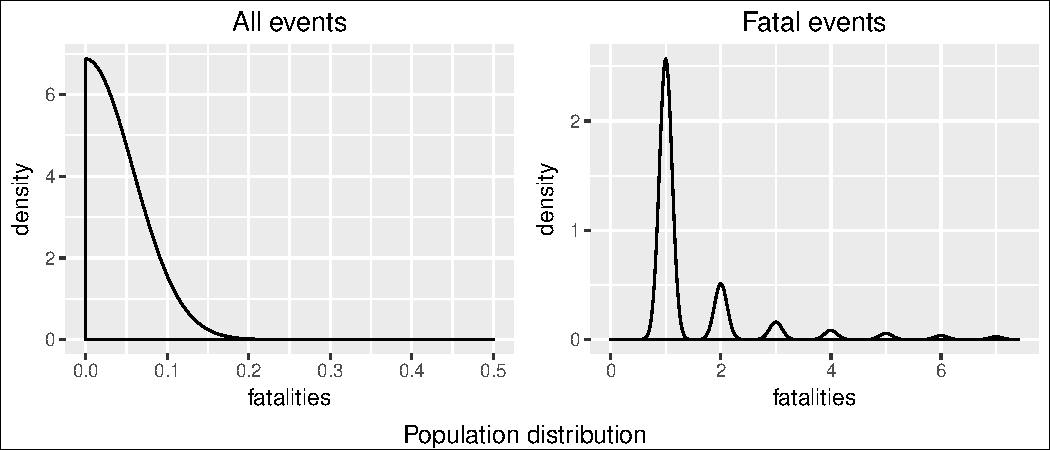
\includegraphics{readme_files/figure-latex/fatal-distr-4-1.pdf}

In this study, we looked on the 1\% deadliest occurrences.

\begin{Shaded}
\begin{Highlighting}[]
\CommentTok{# subset for 99% CI}
\NormalTok{fatal95.df <-}\StringTok{ }\NormalTok{fatal.df %>%}\StringTok{ }\KeywordTok{filter}\NormalTok{(fatalities>qt[}\DecValTok{1}\NormalTok{])}
                
\CommentTok{# create color pallete for all events}
\NormalTok{colourCount.fatal.single =}\StringTok{ }\KeywordTok{length}\NormalTok{(}\KeywordTok{unique}\NormalTok{(fatal95.df$event))}
\NormalTok{getPalette =}\StringTok{ }\KeywordTok{colorRampPalette}\NormalTok{(}\KeywordTok{brewer.pal}\NormalTok{(colourCount.fatal.single, }\StringTok{"Set1"}\NormalTok{))}

\CommentTok{# print a table}
\KeywordTok{kable}\NormalTok{(fatal95.df[, }\KeywordTok{c}\NormalTok{(}\DecValTok{10}\NormalTok{,}\DecValTok{1}\NormalTok{:}\DecValTok{9}\NormalTok{)])}
\end{Highlighting}
\end{Shaded}

\begin{longtable}[]{@{}rlrlrllrrr@{}}
\toprule
rank & event & mag & day & duration & state & countyname & fatalities &
mean & median\tabularnewline
\midrule
\endhead
1 & HEAT & 0 & 1995-07-12 & 0S & IL & ILZ003 & 583 & 2.171638 &
1\tabularnewline
2 & TORNADO & 0 & 2011-05-22 & 0S & MO & JASPER & 158 & 2.171638 &
1\tabularnewline
3 & TORNADO & 0 & 1953-06-08 & NA & MI & GENESEE & 116 & 2.171638 &
1\tabularnewline
4 & TORNADO & 0 & 1953-05-11 & NA & TX & MCLENNAN & 114 & 2.171638 &
1\tabularnewline
5 & HEAT & 0 & 1999-07-28 & 0S & IL & ILZ005 & 99 & 2.171638 &
1\tabularnewline
6 & TORNADO & 0 & 1953-06-09 & NA & MA & WORCESTER & 90 & 2.171638 &
1\tabularnewline
7 & TORNADO & 0 & 1955-05-25 & NA & KS & COWLEY & 75 & 2.171638 &
1\tabularnewline
\bottomrule
\end{longtable}

\begin{Shaded}
\begin{Highlighting}[]
\CommentTok{# prepare text for inline R}
\NormalTok{worst.fatal.single.ev <-}\StringTok{ }\NormalTok{fatal95.df$event[}\DecValTok{1}\NormalTok{]}
\NormalTok{worst.fatal.single.st <-}\StringTok{ }\NormalTok{fatal95.df$state[}\DecValTok{1}\NormalTok{]}
\NormalTok{worst.fatal.single.ct <-}\StringTok{ }\NormalTok{fatal95.df$countyname[}\DecValTok{1}\NormalTok{]}
\NormalTok{worst.fatal.single.dt <-}\StringTok{ }\NormalTok{fatal95.df$day[}\DecValTok{1}\NormalTok{]}
\NormalTok{worst.fatal.single.kill <-}\StringTok{ }\NormalTok{fatal95.df$fatalities[}\DecValTok{1}\NormalTok{]}
\end{Highlighting}
\end{Shaded}

\begin{Shaded}
\begin{Highlighting}[]
\CommentTok{# the plot}
\NormalTok{plt.fatal.single <-}\StringTok{ }\KeywordTok{ggplot}\NormalTok{(fatal95.df, }\KeywordTok{aes}\NormalTok{(day, fatalities, }\DataTypeTok{colour=}\NormalTok{event))}

\NormalTok{plt.fatal.single <-}\StringTok{ }\NormalTok{plt.fatal.single +}\StringTok{ }\KeywordTok{geom_point}\NormalTok{() +}
\StringTok{        }\KeywordTok{geom_text}\NormalTok{(}\KeywordTok{aes}\NormalTok{(}\DataTypeTok{label=}\KeywordTok{ifelse}\NormalTok{(rank <=}\StringTok{ }\DecValTok{3}\NormalTok{,}
                 \KeywordTok{paste0}\NormalTok{(}\KeywordTok{as.character}\NormalTok{(day), }\StringTok{": "}\NormalTok{, fatalities, }\StringTok{" killed"}\NormalTok{) ,}\StringTok{""}\NormalTok{),}
                \DataTypeTok{hjust=}\NormalTok{-.}\DecValTok{03}\NormalTok{,}\DataTypeTok{vjust=}\FloatTok{0.5}\NormalTok{)) +}

\StringTok{        }\CommentTok{# geom_hline(aes(yintercept = mean), linetype=2) +}
\StringTok{        }\CommentTok{# geom_hline(aes(yintercept = median), linetype=3) +}
\StringTok{        }\KeywordTok{labs}\NormalTok{(}\DataTypeTok{title=}\StringTok{"Most Fatal"}\NormalTok{,}
                    \DataTypeTok{y=}\StringTok{""}\NormalTok{, }\DataTypeTok{x=}\StringTok{""}\NormalTok{) +}
\StringTok{    }
\StringTok{        }\KeywordTok{expand_limits}\NormalTok{(}\DataTypeTok{x=}\KeywordTok{as.Date}\NormalTok{(}\StringTok{'2017-01-01'}\NormalTok{))+}\StringTok{ }\CommentTok{#ok}
\StringTok{        }\KeywordTok{scale_colour_manual}\NormalTok{(}\DataTypeTok{values =} \KeywordTok{getPalette}\NormalTok{(colourCount.fatal.single))+}\StringTok{                }
\StringTok{        }\KeywordTok{theme}\NormalTok{(}\DataTypeTok{legend.title=}\KeywordTok{element_blank}\NormalTok{()) +}
\StringTok{        }\KeywordTok{theme}\NormalTok{(}\DataTypeTok{legend.position=}\StringTok{"bottom"}\NormalTok{) +}
\StringTok{        }\KeywordTok{guides}\NormalTok{(}\DataTypeTok{fill=}\KeywordTok{guide_legend}\NormalTok{(}\DataTypeTok{nrow=}\DecValTok{5}\NormalTok{, }\DataTypeTok{byrow=}\OtherTok{TRUE}\NormalTok{)) +}
\StringTok{        }\KeywordTok{theme}\NormalTok{(}\DataTypeTok{axis.text.x =} \KeywordTok{element_text}\NormalTok{(}\DataTypeTok{angle =} \DecValTok{90}\NormalTok{, }\DataTypeTok{hjust =} \DecValTok{1}\NormalTok{)) +}\StringTok{ }
\StringTok{        }\KeywordTok{theme}\NormalTok{(}\DataTypeTok{plot.title =} \KeywordTok{element_text}\NormalTok{(}\DataTypeTok{hjust =} \FloatTok{0.5}\NormalTok{))                 }

\NormalTok{plt.fatal.single +}\StringTok{ }\KeywordTok{labs}\NormalTok{(}\DataTypeTok{title=}\StringTok{"Most fatal Occurrence"}\NormalTok{,}
                    \DataTypeTok{y=}\StringTok{"Fatalities"}\NormalTok{, }\DataTypeTok{x=}\StringTok{""}\NormalTok{)}
\end{Highlighting}
\end{Shaded}

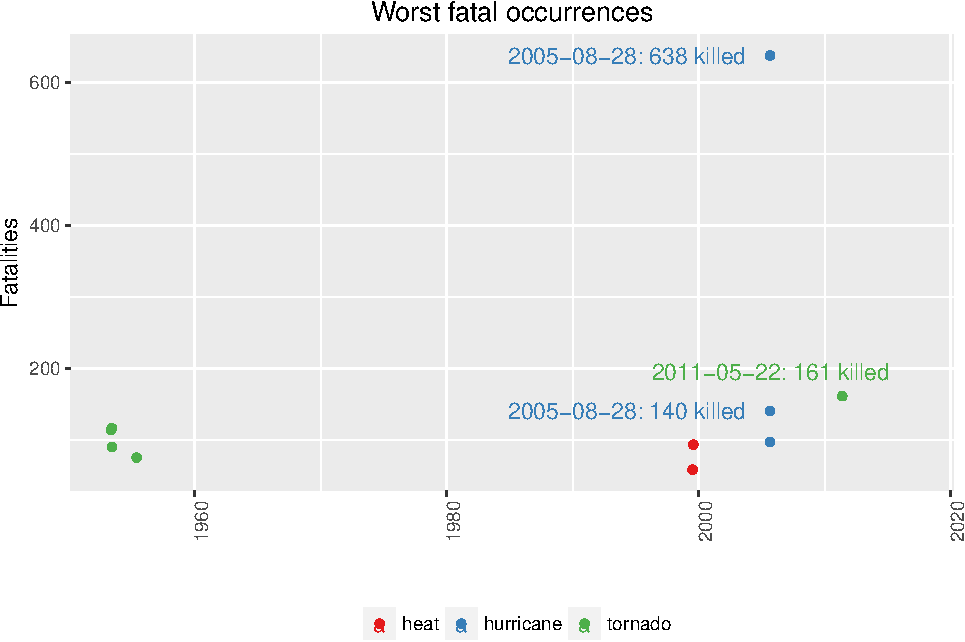
\includegraphics{readme_files/figure-latex/fatal-plot-single-1.pdf}

The single most fatal event was a \textbf{HEAT, that occurred in IL,
ILZ003, on 1995-07-12, killing 583 people.}

However, if we compare this single awful event to the mean of fatalities
caused, we see that this is very unlikely to happen.

\subsection{Most fatal in all time}\label{most-fatal-in-all-time}

Most fatal in all time

Notice that are several occurrences of the same type of event along the
time.

Therefore, in order to know which is the worst type of event along all
the years, we summed up the fatalities caused by each one of occurrences
of this events.

Notice that we are interested only in the worst of them, ie, the ones
which are above the mean.

\begin{Shaded}
\begin{Highlighting}[]
\CommentTok{# totals per event}
\NormalTok{fatal.all.df <-}\StringTok{ }\NormalTok{fatal.df %>%}\StringTok{ }\KeywordTok{group_by}\NormalTok{(event) %>%}
\StringTok{        }\KeywordTok{summarise}\NormalTok{(}\DataTypeTok{total =} \KeywordTok{sum}\NormalTok{(fatalities)) %>%}\StringTok{ }\KeywordTok{arrange}\NormalTok{(}\KeywordTok{desc}\NormalTok{(total)) %>%}\StringTok{ }
\StringTok{        }\KeywordTok{mutate}\NormalTok{(}\DataTypeTok{mean =} \KeywordTok{mean}\NormalTok{(total), }\DataTypeTok{median =} \KeywordTok{median}\NormalTok{(total),}
               \DataTypeTok{rank =} \KeywordTok{seq_len}\NormalTok{(}\KeywordTok{length}\NormalTok{(event))) %>%}
\StringTok{        }\KeywordTok{filter}\NormalTok{(total >}\StringTok{ }\KeywordTok{mean}\NormalTok{(total))}

\CommentTok{# create color pallete for all events}
\NormalTok{colourCount.fatal.all =}\StringTok{ }\KeywordTok{length}\NormalTok{(}\KeywordTok{unique}\NormalTok{(fatal.all.df$event))}
\NormalTok{getPalette =}\StringTok{ }\KeywordTok{colorRampPalette}\NormalTok{(}\KeywordTok{brewer.pal}\NormalTok{(colourCount.fatal.all, }\StringTok{"Set1"}\NormalTok{))}

\CommentTok{# prepare text for inline R}
\NormalTok{worst.fatal.all.ev <-}\StringTok{ }\NormalTok{fatal.all.df$event[}\DecValTok{1}\NormalTok{]}
\NormalTok{worst.fatal.all.kill <-}\StringTok{ }\NormalTok{fatal.all.df$total[}\DecValTok{1}\NormalTok{]}

\CommentTok{# a table}
\KeywordTok{kable}\NormalTok{(fatal.all.df[,}\KeywordTok{c}\NormalTok{(}\DecValTok{5}\NormalTok{,}\DecValTok{1}\NormalTok{:}\DecValTok{4}\NormalTok{)])}
\end{Highlighting}
\end{Shaded}

\begin{longtable}[]{@{}rlrrr@{}}
\toprule
rank & event & total & mean & median\tabularnewline
\midrule
\endhead
1 & TORNADO & 5636 & 398.5526 & 38.5\tabularnewline
2 & HEAT & 3149 & 398.5526 & 38.5\tabularnewline
3 & FLOOD & 1553 & 398.5526 & 38.5\tabularnewline
4 & WIND & 1451 & 398.5526 & 38.5\tabularnewline
5 & LIGHTNING & 816 & 398.5526 & 38.5\tabularnewline
\bottomrule
\end{longtable}

\begin{Shaded}
\begin{Highlighting}[]
\CommentTok{# the plot}
\NormalTok{plt.fatal.all <-}\StringTok{ }\KeywordTok{ggplot}\NormalTok{(}\DataTypeTok{data=}\NormalTok{fatal.all.df, }\KeywordTok{aes}\NormalTok{(event, total, }\DataTypeTok{fill=}\NormalTok{event))}

\NormalTok{plt.fatal.all <-}\StringTok{ }\NormalTok{plt.fatal.all +}\StringTok{ }\KeywordTok{geom_bar}\NormalTok{(}\DataTypeTok{stat=}\StringTok{"identity"}\NormalTok{) +}
\StringTok{        }\KeywordTok{geom_text}\NormalTok{(}\KeywordTok{aes}\NormalTok{(}\DataTypeTok{label=}\KeywordTok{ifelse}\NormalTok{(total==}\KeywordTok{max}\NormalTok{(total),}
                \KeywordTok{paste0}\NormalTok{(event, }\StringTok{": "}\NormalTok{, }\KeywordTok{max}\NormalTok{(total), }\StringTok{" killed"}\NormalTok{),}\StringTok{''}\NormalTok{)),}
                \DataTypeTok{hjust=}\DecValTok{0}\NormalTok{,}\DataTypeTok{vjust=}\DecValTok{2}\NormalTok{) +}
\StringTok{        }\KeywordTok{geom_hline}\NormalTok{(}\KeywordTok{aes}\NormalTok{(}\DataTypeTok{yintercept =} \NormalTok{mean), }\DataTypeTok{linetype=}\DecValTok{1}\NormalTok{) +}
\StringTok{        }\CommentTok{# geom_hline(aes(yintercept = median), linetype=2) +}
\StringTok{        }\KeywordTok{labs}\NormalTok{(}\DataTypeTok{title=}\StringTok{"All time"}\NormalTok{, }\DataTypeTok{y=}\StringTok{""}\NormalTok{,}
             \DataTypeTok{x=}\StringTok{""}\NormalTok{) +}\StringTok{ }
\StringTok{                }
\StringTok{        }\KeywordTok{theme}\NormalTok{(}\DataTypeTok{legend.position=}\StringTok{"none"}\NormalTok{) +}\StringTok{        }
\StringTok{        }\KeywordTok{scale_colour_manual}\NormalTok{(}\DataTypeTok{values =} \KeywordTok{getPalette}\NormalTok{(colourCount.fatal.all))+}\StringTok{                }
\StringTok{        }\KeywordTok{theme}\NormalTok{(}\DataTypeTok{legend.title=}\KeywordTok{element_blank}\NormalTok{()) +}
\StringTok{        }\KeywordTok{theme}\NormalTok{(}\DataTypeTok{axis.text.x =} \KeywordTok{element_text}\NormalTok{(}\DataTypeTok{angle =} \DecValTok{90}\NormalTok{, }\DataTypeTok{hjust =} \DecValTok{1}\NormalTok{)) +}\StringTok{ }
\StringTok{        }\KeywordTok{theme}\NormalTok{(}\DataTypeTok{plot.title =} \KeywordTok{element_text}\NormalTok{(}\DataTypeTok{hjust =} \FloatTok{0.5}\NormalTok{))                 }

\NormalTok{plt.fatal.all +}\StringTok{ }\KeywordTok{labs}\NormalTok{(}\DataTypeTok{title=}\StringTok{"Most fatal type of event - all time"}\NormalTok{,}
                    \DataTypeTok{y=}\StringTok{"Fatalities"}\NormalTok{, }\DataTypeTok{x=}\StringTok{""}\NormalTok{)                }
\end{Highlighting}
\end{Shaded}

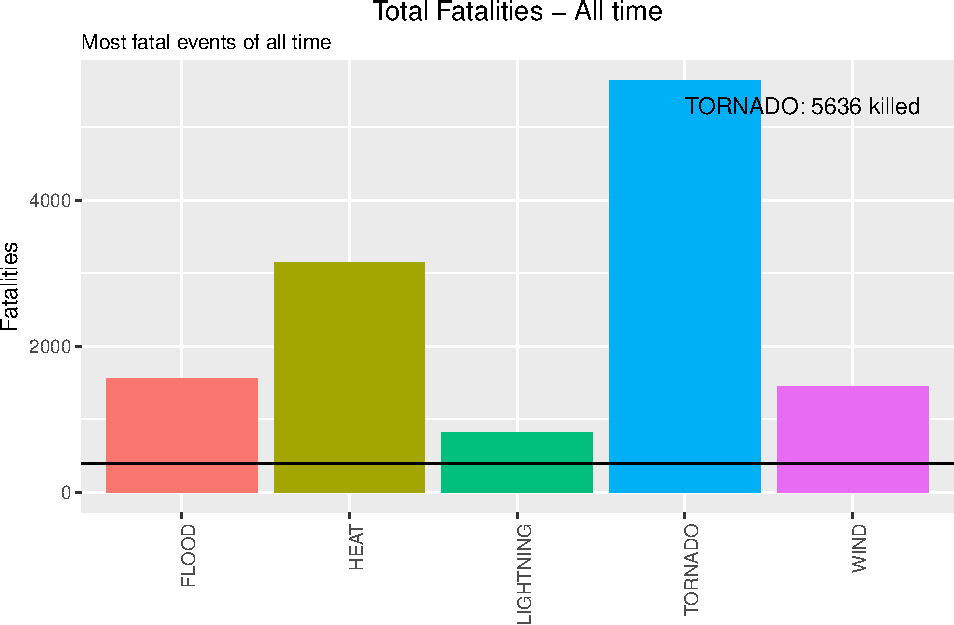
\includegraphics{readme_files/figure-latex/fatal-plot-alltime-1.pdf}

The most fatal event along the time is the \textbf{TORNADO. It has
killed 5636 people until now.}

Just for curiosity, these are the less fatal among the fatal events:

\begin{Shaded}
\begin{Highlighting}[]
\CommentTok{# sort for less dangerous, had to subset again due to previous filtering}
\NormalTok{fatal.all.df <-}\StringTok{ }\NormalTok{fatal.df %>%}\StringTok{ }\KeywordTok{group_by}\NormalTok{(event) %>%}
\StringTok{        }\KeywordTok{summarise}\NormalTok{(}\DataTypeTok{total =} \KeywordTok{sum}\NormalTok{(fatalities)) %>%}\StringTok{ }\KeywordTok{arrange}\NormalTok{(total) %>%}\StringTok{ }
\StringTok{        }\KeywordTok{mutate}\NormalTok{(}\DataTypeTok{mean =} \KeywordTok{mean}\NormalTok{(total), }\DataTypeTok{median =} \KeywordTok{median}\NormalTok{(total),}
               \DataTypeTok{rank =} \KeywordTok{seq}\NormalTok{(}\KeywordTok{length}\NormalTok{(event),}\DecValTok{1}\NormalTok{, }\DataTypeTok{by=}\NormalTok{-}\DecValTok{1}\NormalTok{))}

\CommentTok{# a table}
\KeywordTok{kable}\NormalTok{(fatal.all.df[}\DecValTok{1}\NormalTok{:}\DecValTok{10}\NormalTok{,}\KeywordTok{c}\NormalTok{(}\DecValTok{5}\NormalTok{,}\DecValTok{1}\NormalTok{:}\DecValTok{2}\NormalTok{)])}
\end{Highlighting}
\end{Shaded}

\begin{longtable}[]{@{}rlr@{}}
\toprule
rank & event & total\tabularnewline
\midrule
\endhead
38 & BLACK ICE & 1\tabularnewline
37 & FROST & 1\tabularnewline
36 & HIGH SWELLS & 1\tabularnewline
35 & WINTRY MIX & 1\tabularnewline
34 & DUST DEVIL & 2\tabularnewline
33 & SLEET & 2\tabularnewline
32 & HIGH WATER & 3\tabularnewline
31 & WATERSPOUT & 3\tabularnewline
30 & HIGH SEAS & 5\tabularnewline
29 & ICY ROADS & 5\tabularnewline
\bottomrule
\end{longtable}

\subsection{Injuring Occurrences}\label{injuring-occurrences}

\subsection{Most injuring in a single
occurrence}\label{most-injuring-in-a-single-occurrence}

Most injuring in a single occurrence

In order to determine what were the most injuring events in a single
occurrence, we need to see how injuries are distributed along the
occurrences.

\begin{Shaded}
\begin{Highlighting}[]
\KeywordTok{rm}\NormalTok{(fatal.df,fatal.all.df, fatal95.df, qt) }\CommentTok{# cleannig house}


\NormalTok{injuring.df <-}\StringTok{ }\NormalTok{harm.df %>%}\StringTok{ }\KeywordTok{filter}\NormalTok{(!}\KeywordTok{is.na}\NormalTok{(injuries)) %>%}
\StringTok{                }\KeywordTok{select}\NormalTok{(}\DecValTok{1}\NormalTok{:}\DecValTok{6}\NormalTok{,}\DecValTok{8}\NormalTok{)}

\CommentTok{# quantiles}
\NormalTok{qt <-}\StringTok{ }\KeywordTok{quantile}\NormalTok{(injuring.df$injuries, }\DataTypeTok{probs=}\KeywordTok{seq}\NormalTok{(.}\DecValTok{975}\NormalTok{,}\DecValTok{1}\NormalTok{,}\FloatTok{0.002}\NormalTok{))}

\CommentTok{# distribution plot}
\NormalTok{plt.distr.inj0 <-}\StringTok{ }\KeywordTok{ggplot}\NormalTok{(injuring.df, }\KeywordTok{aes}\NormalTok{(injuries))}

\NormalTok{plt.distr.inj0 <-}\StringTok{ }\NormalTok{plt.distr.inj0 +}\StringTok{ }\KeywordTok{geom_density}\NormalTok{(}\KeywordTok{aes}\NormalTok{(}\DataTypeTok{y=}\NormalTok{..density..)) +}\StringTok{ }\KeywordTok{xlim}\NormalTok{(}\DecValTok{0}\NormalTok{,}\FloatTok{0.5}\NormalTok{) +}\StringTok{ }
\StringTok{        }\KeywordTok{labs}\NormalTok{(}\DataTypeTok{title=}\StringTok{"All events"}\NormalTok{) +}
\StringTok{        }\KeywordTok{theme}\NormalTok{(}\DataTypeTok{plot.title =} \KeywordTok{element_text}\NormalTok{(}\DataTypeTok{hjust =} \FloatTok{0.5}\NormalTok{))}


\CommentTok{# display only the qts next to injuring events}
\NormalTok{qt[(}\KeywordTok{length}\NormalTok{(qt)-(}\KeywordTok{length}\NormalTok{(qt[qt>=}\DecValTok{1}\NormalTok{])+}\DecValTok{1}\NormalTok{)):}\StringTok{ }\KeywordTok{length}\NormalTok{(qt)]}
\end{Highlighting}
\end{Shaded}

\begin{verbatim}
## 97.7% 97.9% 98.1% 98.3% 98.5% 98.7% 98.9% 99.1% 99.3% 99.5% 99.7% 99.9% 
##     0     0     1     1     1     1     1     2     3     4     8    25
\end{verbatim}

Looking at this distribution, we can infer that the vast majority of
those occurrences were not injuring at all: \textbf{97.9\% occurrences
didn't caused any injuries}

On the other hand, injuring occurrences had to have at least 1 injury.

Now, among the injuring occurrences, we are interested in the ones whose
harm is beyond the confidence interval, ie. above 99\% of the most
common values.

\begin{Shaded}
\begin{Highlighting}[]
\CommentTok{# subset for harm events}
\NormalTok{injuring.df <-}\StringTok{ }\NormalTok{injuring.df %>%}\StringTok{ }\KeywordTok{filter}\NormalTok{(injuries >}\StringTok{ }\DecValTok{0}\NormalTok{) %>%}
\StringTok{                }\KeywordTok{arrange}\NormalTok{(}\KeywordTok{desc}\NormalTok{(injuries)) %>%}
\StringTok{                }\KeywordTok{mutate}\NormalTok{(}\DataTypeTok{mean =} \KeywordTok{mean}\NormalTok{(injuries), }
                \DataTypeTok{median =} \KeywordTok{median}\NormalTok{(injuries),}
                \DataTypeTok{rank =} \KeywordTok{seq_len}\NormalTok{(}\KeywordTok{length}\NormalTok{(event)))}

\CommentTok{# quantiles, same as }
\CommentTok{# poisson.test(mean, conf.level = 0.95)}

\NormalTok{qt <-}\StringTok{ }\KeywordTok{quantile}\NormalTok{(injuring.df$injuries, }\DataTypeTok{probs=}\KeywordTok{seq}\NormalTok{(.}\DecValTok{999}\NormalTok{,}\DecValTok{1}\NormalTok{,}\FloatTok{0.005}\NormalTok{))}
\NormalTok{qt}
\end{Highlighting}
\end{Shaded}

\begin{verbatim}
## 99.9% 
##   500
\end{verbatim}

Looking at this distribution, we can infer that \textbf{99.8\% of the
injuring occurrences caused up to 500 injuries}.

Distribution plots

\begin{Shaded}
\begin{Highlighting}[]
\CommentTok{# distribution plot}
\NormalTok{plt.distr.inj1 <-}\StringTok{ }\KeywordTok{ggplot}\NormalTok{(injuring.df, }\KeywordTok{aes}\NormalTok{(injuries))}

\NormalTok{plt.distr.inj1 <-}\StringTok{ }\NormalTok{plt.distr.inj1 +}\StringTok{ }\KeywordTok{geom_density}\NormalTok{(}\KeywordTok{aes}\NormalTok{(}\DataTypeTok{y=}\NormalTok{..density..)) +}\StringTok{ }\KeywordTok{xlim}\NormalTok{(}\DecValTok{0}\NormalTok{,(qt[}\DecValTok{1}\NormalTok{]/}\DecValTok{20}\NormalTok{)) +}\StringTok{ }
\StringTok{        }\KeywordTok{labs}\NormalTok{(}\DataTypeTok{title=}\StringTok{"Injuring events"}\NormalTok{) +}
\StringTok{        }\KeywordTok{theme}\NormalTok{(}\DataTypeTok{plot.title =} \KeywordTok{element_text}\NormalTok{(}\DataTypeTok{hjust =} \FloatTok{0.5}\NormalTok{))       }
\end{Highlighting}
\end{Shaded}

\begin{Shaded}
\begin{Highlighting}[]
\KeywordTok{grid.arrange}\NormalTok{(plt.distr.inj0, plt.distr.inj1,}
             \DataTypeTok{nrow=}\DecValTok{1}\NormalTok{, }\DataTypeTok{ncol=}\DecValTok{2}\NormalTok{, }
             \DataTypeTok{bottom=}\StringTok{"Population distribution"}\NormalTok{)}
\KeywordTok{grid.rect}\NormalTok{(}\DataTypeTok{gp=}\KeywordTok{gpar}\NormalTok{(}\DataTypeTok{fill=}\OtherTok{NA}\NormalTok{))}
\end{Highlighting}
\end{Shaded}

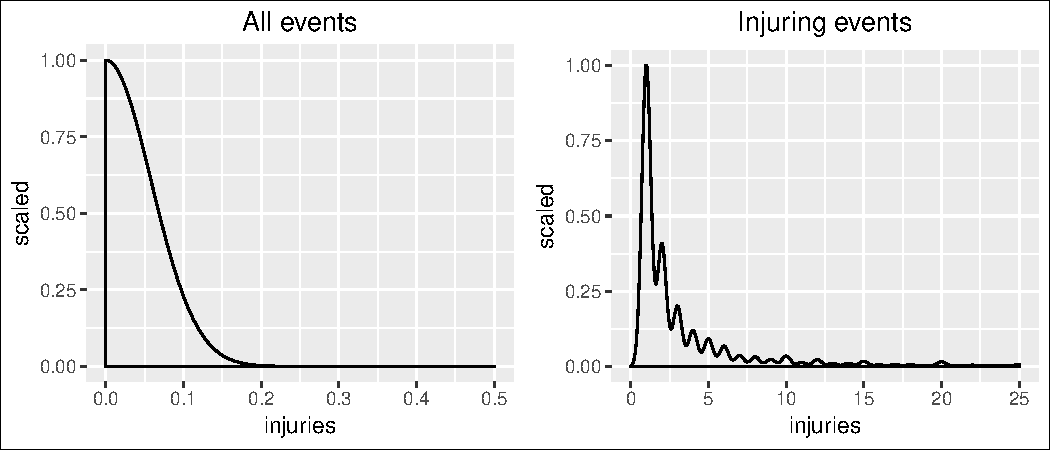
\includegraphics{readme_files/figure-latex/inj-distribution-1.pdf}

In this study, we looked on the 1\% most injuring occurrences.

\begin{Shaded}
\begin{Highlighting}[]
\CommentTok{# subset for 99% CI}
\NormalTok{injuring95.df <-}\StringTok{ }\KeywordTok{filter}\NormalTok{(injuring.df, injuries>qt[}\DecValTok{1}\NormalTok{])}

\CommentTok{# create color pallete for all events}
\NormalTok{colourCount.inj.single =}\StringTok{ }\KeywordTok{length}\NormalTok{(}\KeywordTok{unique}\NormalTok{(injuring95.df$event))}
\NormalTok{getPalette =}\StringTok{ }\KeywordTok{colorRampPalette}\NormalTok{(}\KeywordTok{brewer.pal}\NormalTok{(colourCount.inj.single, }\StringTok{"Set1"}\NormalTok{))}

\CommentTok{# print a table}
\KeywordTok{kable}\NormalTok{(injuring95.df[,}\KeywordTok{c}\NormalTok{(}\DecValTok{10}\NormalTok{,}\DecValTok{1}\NormalTok{:}\DecValTok{9}\NormalTok{)])}
\end{Highlighting}
\end{Shaded}

\begin{longtable}[]{@{}rlrlrllrrr@{}}
\toprule
rank & event & mag & day & duration & state & countyname & injuries &
mean & median\tabularnewline
\midrule
\endhead
1 & TORNADO & 0 & 1979-04-10 & NA & TX & WICHITA & 1700 & 7.982731 &
2\tabularnewline
2 & STORM & 0 & 1994-02-08 & 0S & OH & OHZ42 & 1568 & 7.982731 &
2\tabularnewline
3 & TORNADO & 0 & 1953-06-09 & NA & MA & WORCESTER & 1228 & 7.982731 &
2\tabularnewline
4 & TORNADO & 0 & 1974-04-03 & NA & OH & GREENE & 1150 & 7.982731 &
2\tabularnewline
5 & TORNADO & 0 & 2011-05-22 & 0S & MO & JASPER & 1150 & 7.982731 &
2\tabularnewline
6 & FLOOD & 0 & 1998-10-17 & 0S & TX & COMAL & 800 & 7.982731 &
2\tabularnewline
7 & TORNADO & 0 & 2011-04-27 & 0S & AL & TUSCALOOS & 800 & 7.982731 &
2\tabularnewline
8 & TORNADO & 0 & 1953-06-08 & NA & MI & GENESEE & 785 & 7.982731 &
2\tabularnewline
9 & HURRICANE & 0 & 2004-08-13 & 0S & FL & FLZ055 & 780 & 7.982731 &
2\tabularnewline
10 & FLOOD & 0 & 1998-10-17 & 0S & TX & TXZ206 & 750 & 7.982731 &
2\tabularnewline
11 & TORNADO & 0 & 2011-04-27 & 0S & AL & JEFFERSON & 700 & 7.982731 &
2\tabularnewline
12 & FLOOD & 0 & 1998-10-17 & 0S & TX & BEXAR & 600 & 7.982731 &
2\tabularnewline
13 & TORNADO & 0 & 1953-05-11 & NA & TX & MCLENNAN & 597 & 7.982731 &
2\tabularnewline
14 & TORNADO & 0 & 1965-04-11 & NA & IN & HOWARD & 560 & 7.982731 &
2\tabularnewline
15 & FLOOD & 0 & 1998-10-17 & 0S & TX & TXZ205 & 550 & 7.982731 &
2\tabularnewline
16 & HEAT & 0 & 2007-08-04 & 0S & MO & MOZ061 & 519 & 7.982731 &
2\tabularnewline
17 & TORNADO & 0 & 1966-03-03 & NA & MS & HINDS & 504 & 7.982731 &
2\tabularnewline
\bottomrule
\end{longtable}

\begin{Shaded}
\begin{Highlighting}[]
\CommentTok{# prepare text for inline R}
\NormalTok{worst.injuring.single.ev <-}\StringTok{ }\NormalTok{injuring95.df$event[}\DecValTok{1}\NormalTok{]}
\NormalTok{worst.injuring.single.st <-}\StringTok{ }\NormalTok{injuring95.df$state[}\DecValTok{1}\NormalTok{]}
\NormalTok{worst.injuring.single.ct <-}\StringTok{ }\NormalTok{injuring95.df$countyname[}\DecValTok{1}\NormalTok{]}
\NormalTok{worst.injuring.single.dt <-}\StringTok{ }\NormalTok{injuring95.df$day[}\DecValTok{1}\NormalTok{]}
\NormalTok{worst.injuring.single.inj <-}\StringTok{ }\NormalTok{injuring95.df$injuries[}\DecValTok{1}\NormalTok{]}
\end{Highlighting}
\end{Shaded}

\begin{Shaded}
\begin{Highlighting}[]
\CommentTok{# the plot}
\NormalTok{plt.inj.single <-}\StringTok{ }\KeywordTok{ggplot}\NormalTok{(injuring95.df, }\KeywordTok{aes}\NormalTok{(day, injuries, }\DataTypeTok{colour=}\NormalTok{event))}

\NormalTok{plt.inj.single <-}\StringTok{ }\NormalTok{plt.inj.single +}\StringTok{ }\KeywordTok{geom_point}\NormalTok{() +}
\StringTok{        }\KeywordTok{geom_text}\NormalTok{(}\KeywordTok{aes}\NormalTok{(}\DataTypeTok{label=}\KeywordTok{ifelse}\NormalTok{(rank <=}\StringTok{ }\DecValTok{3}\NormalTok{,}
                 \KeywordTok{paste0}\NormalTok{(}\KeywordTok{as.character}\NormalTok{(day), }\StringTok{": "}\NormalTok{, injuries, }\StringTok{" injuried"}\NormalTok{) ,}\StringTok{""}\NormalTok{),}
                \DataTypeTok{hjust=}\NormalTok{-.}\DecValTok{03}\NormalTok{,}\DataTypeTok{vjust=}\FloatTok{0.5}\NormalTok{)) +}

\StringTok{        }\CommentTok{# geom_hline(aes(yintercept = mean), linetype=2) +}
\StringTok{        }\CommentTok{# geom_hline(aes(yintercept = median), linetype=3) +}
\StringTok{        }\KeywordTok{labs}\NormalTok{(}\DataTypeTok{title=}\StringTok{"Most Injuring"}\NormalTok{,}
                    \DataTypeTok{y=}\StringTok{""}\NormalTok{, }\DataTypeTok{x=}\StringTok{""}\NormalTok{) +}
\StringTok{                }
\StringTok{        }\KeywordTok{expand_limits}\NormalTok{(}\DataTypeTok{x=}\KeywordTok{as.Date}\NormalTok{(}\StringTok{'2017-01-01'}\NormalTok{))+}\StringTok{ }\CommentTok{#ok}
\StringTok{        }\KeywordTok{scale_colour_manual}\NormalTok{(}\DataTypeTok{values =} \KeywordTok{getPalette}\NormalTok{(colourCount.inj.single))+}\StringTok{                }
\StringTok{        }\KeywordTok{theme}\NormalTok{(}\DataTypeTok{legend.title=}\KeywordTok{element_blank}\NormalTok{()) +}
\StringTok{        }\KeywordTok{theme}\NormalTok{(}\DataTypeTok{legend.position=}\StringTok{"bottom"}\NormalTok{) +}
\StringTok{        }\KeywordTok{guides}\NormalTok{(}\DataTypeTok{fill=}\KeywordTok{guide_legend}\NormalTok{(}\DataTypeTok{nrow=}\DecValTok{5}\NormalTok{, }\DataTypeTok{byrow=}\OtherTok{TRUE}\NormalTok{)) +}
\StringTok{        }\KeywordTok{theme}\NormalTok{(}\DataTypeTok{axis.text.x =} \KeywordTok{element_text}\NormalTok{(}\DataTypeTok{angle =} \DecValTok{90}\NormalTok{, }\DataTypeTok{hjust =} \DecValTok{1}\NormalTok{)) +}\StringTok{ }
\StringTok{        }\KeywordTok{theme}\NormalTok{(}\DataTypeTok{plot.title =} \KeywordTok{element_text}\NormalTok{(}\DataTypeTok{hjust =} \FloatTok{0.5}\NormalTok{)) }

\NormalTok{plt.inj.single +}\StringTok{ }\KeywordTok{labs}\NormalTok{(}\DataTypeTok{title=}\StringTok{"Most Injuring Occurrence"}\NormalTok{,}
                    \DataTypeTok{y=}\StringTok{"Injuries"}\NormalTok{, }\DataTypeTok{x=}\StringTok{""}\NormalTok{) }
\end{Highlighting}
\end{Shaded}

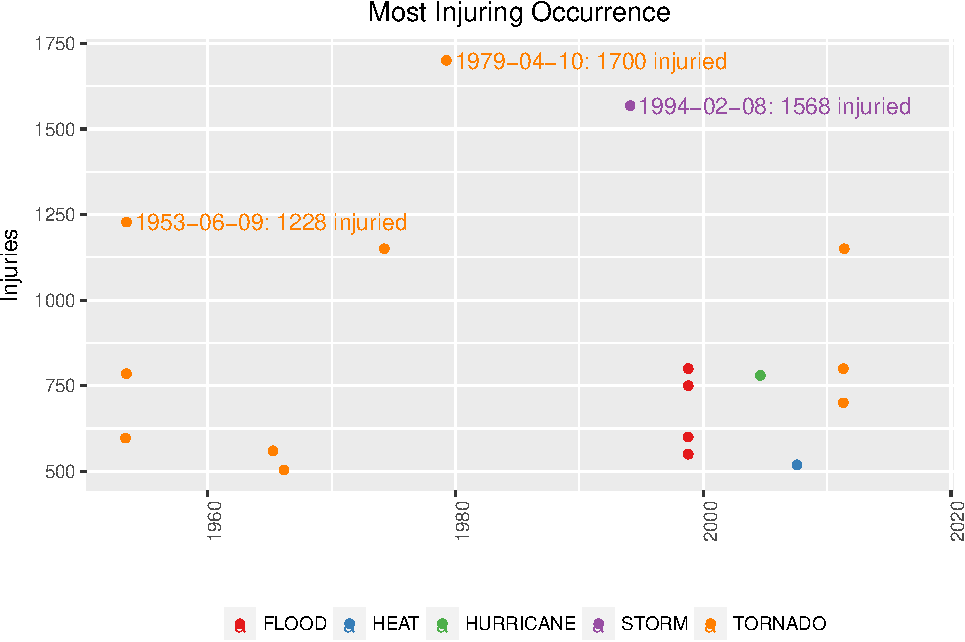
\includegraphics{readme_files/figure-latex/injuring-single-plot-1.pdf}

\begin{Shaded}
\begin{Highlighting}[]
        \CommentTok{# scale_y_continuous(expand = c(0, 0)) +}
        \CommentTok{# geom_hline(aes(yintercept = mean), linetype=2) +}
        \CommentTok{# geom_hline(aes(yintercept = median), linetype=3)}
\end{Highlighting}
\end{Shaded}

The single most injuring event was a \textbf{TORNADO, that occurred in
TX, WICHITA, on 1979-04-10, injuring 1700 people.}

However, if we compare this single awful event to the mean of injuries
caused, we see that this is very unlikely to happen.

\subsection{Most injuring in all time}\label{most-injuring-in-all-time}

Most injuring in all time

Notice that are several occurrences of the same type of event along the
time.

Therefore, in order to know which is the worst type of event along all
the years, we summed up the injuries caused by each one of occurrences
of this events.

Notice that we are interested only in the worst of them, ie, the ones
which are above the mean.

\begin{Shaded}
\begin{Highlighting}[]
\CommentTok{# totals per event}
\NormalTok{injuring.all.df <-}\StringTok{ }\NormalTok{injuring.df %>%}\StringTok{ }\KeywordTok{group_by}\NormalTok{(event) %>%}\StringTok{ }
\StringTok{        }\KeywordTok{summarise}\NormalTok{(}\DataTypeTok{total =} \KeywordTok{sum}\NormalTok{(injuries)) %>%}
\StringTok{        }\KeywordTok{arrange}\NormalTok{(}\KeywordTok{desc}\NormalTok{(total)) %>%}\StringTok{ }
\StringTok{        }\KeywordTok{mutate}\NormalTok{(}\DataTypeTok{mean =} \KeywordTok{mean}\NormalTok{(total), }\DataTypeTok{median =} \KeywordTok{median}\NormalTok{(total),}
               \DataTypeTok{rank =} \KeywordTok{seq_len}\NormalTok{(}\KeywordTok{length}\NormalTok{(event)))  %>%}
\StringTok{        }\KeywordTok{filter}\NormalTok{(total >=}\StringTok{ }\KeywordTok{mean}\NormalTok{(total))}

\CommentTok{# create color pallete for all events}
\NormalTok{colourCount.inj.all =}\StringTok{ }\KeywordTok{length}\NormalTok{(}\KeywordTok{unique}\NormalTok{(injuring.all.df$event))}
\NormalTok{getPalette =}\StringTok{ }\KeywordTok{colorRampPalette}\NormalTok{(}\KeywordTok{brewer.pal}\NormalTok{(colourCount.inj.all, }\StringTok{"Set1"}\NormalTok{))}

\CommentTok{# prepare text for inline R}
\NormalTok{worst.injuring.all.ev <-}\StringTok{ }\NormalTok{injuring.all.df$event[}\DecValTok{1}\NormalTok{]}
\NormalTok{worst.injuring.all.inj <-}\StringTok{ }\NormalTok{injuring.all.df$total[}\DecValTok{1}\NormalTok{]}

\CommentTok{# a table}
\KeywordTok{kable}\NormalTok{(injuring.all.df[,}\KeywordTok{c}\NormalTok{(}\DecValTok{5}\NormalTok{,}\DecValTok{1}\NormalTok{:}\DecValTok{4}\NormalTok{)])}
\end{Highlighting}
\end{Shaded}

\begin{longtable}[]{@{}rlrrr@{}}
\toprule
rank & event & total & mean & median\tabularnewline
\midrule
\endhead
1 & TORNADO & 91407 & 4015.086 & 232\tabularnewline
2 & WIND & 11497 & 4015.086 & 232\tabularnewline
3 & HEAT & 9243 & 4015.086 & 232\tabularnewline
4 & FLOOD & 8683 & 4015.086 & 232\tabularnewline
5 & LIGHTNING & 5230 & 4015.086 & 232\tabularnewline
\bottomrule
\end{longtable}

The most injuring event along the time is the \textbf{TORNADO. It has
injuried 91407 people until now.}

\begin{Shaded}
\begin{Highlighting}[]
\CommentTok{# the plot}
\NormalTok{plt.inj.all <-}\StringTok{ }\KeywordTok{ggplot}\NormalTok{(}\DataTypeTok{data=}\NormalTok{injuring.all.df, }\KeywordTok{aes}\NormalTok{(event, total, }\DataTypeTok{fill=}\NormalTok{event))}

\NormalTok{plt.inj.all <-}\StringTok{ }\NormalTok{plt.inj.all +}\StringTok{ }\KeywordTok{geom_bar}\NormalTok{(}\DataTypeTok{stat=}\StringTok{"identity"}\NormalTok{) +}
\StringTok{        }\KeywordTok{geom_text}\NormalTok{(}\KeywordTok{aes}\NormalTok{(}\DataTypeTok{label=}\KeywordTok{ifelse}\NormalTok{(total==}\KeywordTok{max}\NormalTok{(total),}
                \KeywordTok{paste0}\NormalTok{(event, }\StringTok{": "}\NormalTok{, }\KeywordTok{max}\NormalTok{(total), }\StringTok{" injuried"}\NormalTok{),}\StringTok{''}\NormalTok{)),}
                \DataTypeTok{hjust=}\DecValTok{0}\NormalTok{,}\DataTypeTok{vjust=}\DecValTok{2}\NormalTok{) +}
\StringTok{        }\KeywordTok{geom_hline}\NormalTok{(}\KeywordTok{aes}\NormalTok{(}\DataTypeTok{yintercept =} \NormalTok{mean), }\DataTypeTok{linetype=}\DecValTok{1}\NormalTok{) +}
\StringTok{        }\CommentTok{# geom_hline(aes(yintercept = median), linetype=2) +}
\StringTok{        }\KeywordTok{labs}\NormalTok{(}\DataTypeTok{title=}\StringTok{"All time"}\NormalTok{, }
             \DataTypeTok{y=}\StringTok{""}\NormalTok{, }\DataTypeTok{x=}\StringTok{""}\NormalTok{) +}\StringTok{ }
\StringTok{                }
\StringTok{        }\KeywordTok{theme}\NormalTok{(}\DataTypeTok{legend.position=}\StringTok{"none"}\NormalTok{) +}\StringTok{        }
\StringTok{        }\KeywordTok{scale_colour_manual}\NormalTok{(}\DataTypeTok{values =} \KeywordTok{getPalette}\NormalTok{(colourCount.inj.all))+}\StringTok{                }
\StringTok{        }\KeywordTok{theme}\NormalTok{(}\DataTypeTok{legend.title=}\KeywordTok{element_blank}\NormalTok{()) +}
\StringTok{        }\KeywordTok{theme}\NormalTok{(}\DataTypeTok{axis.text.x =} \KeywordTok{element_text}\NormalTok{(}\DataTypeTok{angle =} \DecValTok{90}\NormalTok{, }\DataTypeTok{hjust =} \DecValTok{1}\NormalTok{)) +}\StringTok{ }
\StringTok{        }\KeywordTok{theme}\NormalTok{(}\DataTypeTok{plot.title =} \KeywordTok{element_text}\NormalTok{(}\DataTypeTok{hjust =} \FloatTok{0.5}\NormalTok{))                 }
                

\NormalTok{plt.inj.all  +}\StringTok{ }\KeywordTok{labs}\NormalTok{(}\DataTypeTok{title=}\StringTok{"Most Injuring type of event - all time"}\NormalTok{,}
                    \DataTypeTok{y=}\StringTok{"Injuries"}\NormalTok{, }\DataTypeTok{x=}\StringTok{""}\NormalTok{)}
\end{Highlighting}
\end{Shaded}

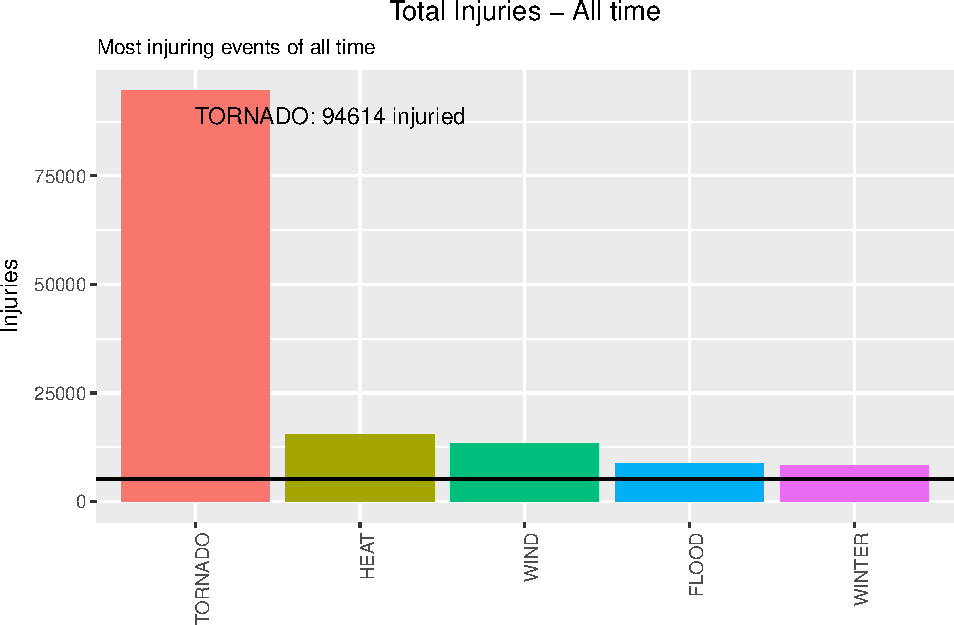
\includegraphics{readme_files/figure-latex/injuring-all-plot-1.pdf}

Just for curiosity, lets show now what are the less injuring among the
injuring events:

\begin{Shaded}
\begin{Highlighting}[]
\CommentTok{# sort for less dangerous, had to subset again due to previous filtering}
\NormalTok{injuring.all.df <-}\StringTok{ }\NormalTok{injuring.df %>%}\StringTok{ }\KeywordTok{group_by}\NormalTok{(event) %>%}
\StringTok{        }\KeywordTok{summarise}\NormalTok{(}\DataTypeTok{total =} \KeywordTok{sum}\NormalTok{(injuries)) %>%}\StringTok{ }\KeywordTok{arrange}\NormalTok{(total) %>%}\StringTok{ }
\StringTok{        }\KeywordTok{mutate}\NormalTok{(}\DataTypeTok{mean =} \KeywordTok{mean}\NormalTok{(total), }\DataTypeTok{median =} \KeywordTok{median}\NormalTok{(total),}
               \DataTypeTok{rank =} \KeywordTok{seq}\NormalTok{(}\KeywordTok{length}\NormalTok{(event),}\DecValTok{1}\NormalTok{, }\DataTypeTok{by=}\NormalTok{-}\DecValTok{1}\NormalTok{))}

\CommentTok{# a table}
\KeywordTok{kable}\NormalTok{(injuring.all.df[}\DecValTok{1}\NormalTok{:}\DecValTok{10}\NormalTok{,}\KeywordTok{c}\NormalTok{(}\DecValTok{5}\NormalTok{,}\DecValTok{1}\NormalTok{:}\DecValTok{2}\NormalTok{)])}
\end{Highlighting}
\end{Shaded}

\begin{longtable}[]{@{}rlr@{}}
\toprule
rank & event & total\tabularnewline
\midrule
\endhead
35 & FROST & 3\tabularnewline
34 & FUNNEL & 3\tabularnewline
33 & TIDE & 5\tabularnewline
32 & TYPHOON & 5\tabularnewline
31 & HIGH SEAS & 8\tabularnewline
30 & OTHER & 21\tabularnewline
29 & BLACK ICE & 24\tabularnewline
28 & WATERSPOUT & 29\tabularnewline
27 & ICY ROADS & 31\tabularnewline
26 & DROUGHT & 33\tabularnewline
\bottomrule
\end{longtable}

\section{Economy: the the most harmfull
events}\label{economy-the-the-most-harmfull-events}

We have determined what events did more harm to economy, both in terms
of property and crops damage.

There were events that causes zero property damage but a lot of crop
damage. The inverse is also true, so we did a separate analysis to
property VS crop damaging events.

\subsection{Property losses}\label{property-losses}

\subsection{Most Property Damaging event in a single
occurrence}\label{most-property-damaging-event-in-a-single-occurrence}

Most Property Damaging event in a single occurrence

In order to determine what were the most property damaging events in a
single occurrence, we need to see how damages are distributed along the
occurrences.

\begin{Shaded}
\begin{Highlighting}[]
\CommentTok{# property damages}
\KeywordTok{rm}\NormalTok{(injuring.df, injuring.all.df, injuring95.df) }\CommentTok{# cleannig house}

\NormalTok{prop.df <-}\StringTok{ }\NormalTok{harm.df %>%}\StringTok{ }\KeywordTok{filter}\NormalTok{(!}\KeywordTok{is.na}\NormalTok{(prop.ev)) %>%}
\StringTok{                        }\KeywordTok{select}\NormalTok{(}\DecValTok{1}\NormalTok{:}\DecValTok{6}\NormalTok{,}\DecValTok{13}\NormalTok{)}
                

\CommentTok{# quantiles}
\NormalTok{qt <-}\StringTok{ }\KeywordTok{quantile}\NormalTok{(prop.df$prop.ev, }\DataTypeTok{probs=}\KeywordTok{seq}\NormalTok{(.}\DecValTok{999}\NormalTok{,}\DecValTok{1}\NormalTok{,}\FloatTok{0.002}\NormalTok{))}

\CommentTok{# distribution plot}
\NormalTok{plt.distr.prop0 <-}\StringTok{ }\KeywordTok{ggplot}\NormalTok{(prop.df, }\KeywordTok{aes}\NormalTok{(}\KeywordTok{log}\NormalTok{(prop.ev)))}

\NormalTok{plt.distr.prop0 <-}\StringTok{ }\NormalTok{plt.distr.prop0 +}\StringTok{ }\KeywordTok{geom_density}\NormalTok{(}\KeywordTok{aes}\NormalTok{(}\DataTypeTok{y=}\NormalTok{..density..)) +}\StringTok{ }\CommentTok{#xlim(0,.5) + }
\StringTok{        }\KeywordTok{labs}\NormalTok{(}\DataTypeTok{title=}\StringTok{"All events"}\NormalTok{, }\DataTypeTok{x=}\StringTok{"log(amount $)"}\NormalTok{) +}
\StringTok{        }\KeywordTok{theme}\NormalTok{(}\DataTypeTok{plot.title =} \KeywordTok{element_text}\NormalTok{(}\DataTypeTok{hjust =} \FloatTok{0.5}\NormalTok{))       }


\CommentTok{# display only the qts next to harmfull events}
\NormalTok{qt}
\end{Highlighting}
\end{Shaded}

\begin{verbatim}
##    99.9% 
## 53931800
\end{verbatim}

Looking at this distribution, we can infer that 99.8\% of the
occurrences caused less than \textbf{\$53,931,800 in losses}.

On the other hand, damaging occurrences had to have damages above zero.

Now, among the damaging occurrences, we are interested in the ones whose
damages are above 99.8\% of the most common values.

\begin{Shaded}
\begin{Highlighting}[]
\CommentTok{# subset for harm events}
\NormalTok{prop.df <-}\StringTok{ }\NormalTok{prop.df %>%}\StringTok{ }\KeywordTok{filter}\NormalTok{(prop.ev >}\StringTok{ }\DecValTok{0}\NormalTok{) %>%}
\StringTok{                }\KeywordTok{arrange}\NormalTok{(}\KeywordTok{desc}\NormalTok{(prop.ev)) %>%}
\StringTok{                }\KeywordTok{mutate}\NormalTok{(}\DataTypeTok{value =} \KeywordTok{dollar}\NormalTok{(prop.ev),}
                        \DataTypeTok{media.raw =} \KeywordTok{mean}\NormalTok{(prop.ev), }
                        \DataTypeTok{mediana.raw =} \KeywordTok{median}\NormalTok{(prop.ev),}
                        \DataTypeTok{mean =} \KeywordTok{dollar}\NormalTok{(media.raw),}
                        \DataTypeTok{median =} \KeywordTok{dollar}\NormalTok{(mediana.raw),}
                        \DataTypeTok{rank =} \KeywordTok{seq_len}\NormalTok{(}\KeywordTok{length}\NormalTok{(event)))}
\CommentTok{# quantiles, same as }

\NormalTok{qt <-}\StringTok{ }\KeywordTok{quantile}\NormalTok{(prop.df$prop.ev, }\DataTypeTok{probs=}\KeywordTok{seq}\NormalTok{(.}\DecValTok{999}\NormalTok{,}\DecValTok{1}\NormalTok{,}\FloatTok{0.002}\NormalTok{))}
\NormalTok{qt}
\end{Highlighting}
\end{Shaded}

\begin{verbatim}
##     99.9% 
## 120000000
\end{verbatim}

Looking at this distribution, we can infer that \textbf{99.8\% of the
damaging occurrences caused up to \$120,000,000 in losses}.

Distribution plots

\begin{Shaded}
\begin{Highlighting}[]
\CommentTok{# distribution plot}
\NormalTok{plt.distr.prop1 <-}\StringTok{ }\KeywordTok{ggplot}\NormalTok{(prop.df, }\KeywordTok{aes}\NormalTok{(}\KeywordTok{log}\NormalTok{(prop.ev)))}

\NormalTok{plt.distr.prop1 <-}\StringTok{ }\NormalTok{plt.distr.prop1 +}\StringTok{ }\KeywordTok{geom_density}\NormalTok{(}\KeywordTok{aes}\NormalTok{(}\DataTypeTok{y=}\NormalTok{..density..)) +}\StringTok{ }\CommentTok{#xlim(0,100) + }
\StringTok{        }\KeywordTok{labs}\NormalTok{(}\DataTypeTok{title=}\StringTok{"Damaging events"}\NormalTok{, }\DataTypeTok{x=}\StringTok{"log(amount $)"}\NormalTok{) +}
\StringTok{        }\KeywordTok{theme}\NormalTok{(}\DataTypeTok{plot.title =} \KeywordTok{element_text}\NormalTok{(}\DataTypeTok{hjust =} \FloatTok{0.5}\NormalTok{))     }
\end{Highlighting}
\end{Shaded}

\begin{Shaded}
\begin{Highlighting}[]
\KeywordTok{grid.arrange}\NormalTok{(plt.distr.prop0, plt.distr.prop1,}
             \DataTypeTok{nrow=}\DecValTok{1}\NormalTok{, }\DataTypeTok{ncol=}\DecValTok{2}\NormalTok{, }
             \DataTypeTok{bottom=}\StringTok{"Population distribution"}\NormalTok{)}
\KeywordTok{grid.rect}\NormalTok{(}\DataTypeTok{gp=}\KeywordTok{gpar}\NormalTok{(}\DataTypeTok{fill=}\OtherTok{NA}\NormalTok{))}
\end{Highlighting}
\end{Shaded}

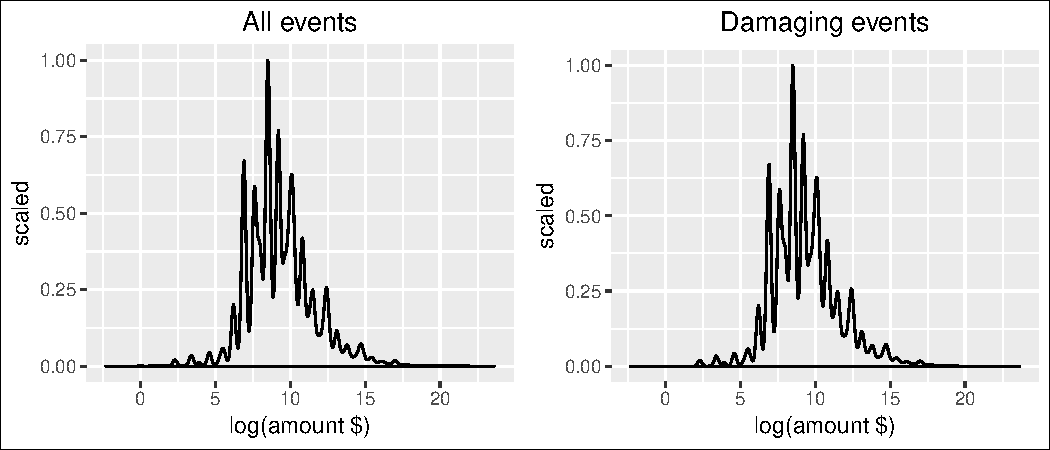
\includegraphics{readme_files/figure-latex/crop-distribution-1.pdf}

In this study, we looked on the 1\% most harmful occurrences.

\begin{Shaded}
\begin{Highlighting}[]
\CommentTok{# subset for 99% CI}
\NormalTok{prop95.df <-}\StringTok{ }\KeywordTok{filter}\NormalTok{(prop.df, prop.ev>qt[}\DecValTok{1}\NormalTok{])}

\CommentTok{# create color pallete for all events}
\NormalTok{colourCount.prop.single =}\StringTok{ }\KeywordTok{length}\NormalTok{(}\KeywordTok{unique}\NormalTok{(prop95.df$event))}
\NormalTok{getPalette =}\StringTok{ }\KeywordTok{colorRampPalette}\NormalTok{(}\KeywordTok{brewer.pal}\NormalTok{(colourCount.prop.single, }\StringTok{"Set1"}\NormalTok{))}


\CommentTok{# print a table}
\KeywordTok{kable}\NormalTok{(prop95.df[}\DecValTok{1}\NormalTok{:}\DecValTok{20}\NormalTok{,}\KeywordTok{c}\NormalTok{(}\DecValTok{13}\NormalTok{,}\DecValTok{1}\NormalTok{:}\DecValTok{6}\NormalTok{,}\DecValTok{8}\NormalTok{,}\DecValTok{11}\NormalTok{:}\DecValTok{12}\NormalTok{)])}
\end{Highlighting}
\end{Shaded}

\begin{longtable}[]{@{}rlrlrlllll@{}}
\toprule
rank & event & mag & day & duration & state & countyname & value & mean
& median\tabularnewline
\midrule
\endhead
1 & FLOOD & 0 & 2006-01-01 & 0S & CA & NAPA & \$115,000,000,000 &
\$1,791,099 & \$10,000\tabularnewline
2 & STORM & 0 & 2005-08-29 & 0S & LA & LAZ040 & \$31,300,000,000 &
\$1,791,099 & \$10,000\tabularnewline
3 & HURRICANE & 0 & 2005-08-28 & 0S & LA & LAZ034 & \$16,930,000,000 &
\$1,791,099 & \$10,000\tabularnewline
4 & STORM & 0 & 2005-08-29 & 0S & MS & MSZ080 & \$11,260,000,000 &
\$1,791,099 & \$10,000\tabularnewline
5 & HURRICANE & 0 & 2005-10-24 & 0S & FL & FLZ068 & \$10,000,000,000 &
\$1,791,099 & \$10,000\tabularnewline
6 & HURRICANE & 0 & 2005-08-28 & 0S & MS & MSZ068 & \$7,350,000,000 &
\$1,791,099 & \$10,000\tabularnewline
7 & HURRICANE & 0 & 2005-08-29 & 0S & MS & MSZ018 & \$5,880,000,000 &
\$1,791,099 & \$10,000\tabularnewline
8 & HURRICANE & 0 & 2004-08-13 & 0S & FL & FLZ055 & \$5,420,000,000 &
\$1,791,099 & \$10,000\tabularnewline
9 & STORM & 0 & 2001-06-05 & 0S & TX & TXZ163 & \$5,150,000,000 &
\$1,791,099 & \$10,000\tabularnewline
10 & WINTER & 0 & 1993-03-12 & 0S & AL & ALZ001 & \$5,000,000,000 &
\$1,791,099 & \$10,000\tabularnewline
11 & FLOOD & 0 & 1993-08-31 & NA & IL & ADAMS & \$5,000,000,000 &
\$1,791,099 & \$10,000\tabularnewline
12 & HURRICANE & 0 & 2004-09-04 & 0S & FL & FLZ041 & \$4,830,000,000 &
\$1,791,099 & \$10,000\tabularnewline
13 & HURRICANE & 0 & 2004-09-13 & 0S & FL & FLZ001 & \$4,000,000,000 &
\$1,791,099 & \$10,000\tabularnewline
14 & HURRICANE & 0 & 2005-09-23 & 0S & LA & LAZ027 & \$4,000,000,000 &
\$1,791,099 & \$10,000\tabularnewline
15 & TIDE & 0 & 2008-09-12 & 0S & TX & TXZ213 & \$4,000,000,000 &
\$1,791,099 & \$10,000\tabularnewline
16 & FLOOD & 0 & 1997-04-18 & 0S & ND & NDZ027 & \$3,000,000,000 &
\$1,791,099 & \$10,000\tabularnewline
17 & HURRICANE & 0 & 1999-09-15 & 0S & NC & NCZ007 & \$3,000,000,000 &
\$1,791,099 & \$10,000\tabularnewline
18 & TORNADO & 0 & 2011-05-22 & 0S & MO & JASPER & \$2,800,000,000 &
\$1,791,099 & \$10,000\tabularnewline
19 & RAIN & 0 & 1995-05-08 & 0S & LA & LAFOURCHE & \$2,500,000,000 &
\$1,791,099 & \$10,000\tabularnewline
20 & HURRICANE & 0 & 2004-09-13 & 0S & AL & ALZ051 & \$2,500,000,000 &
\$1,791,099 & \$10,000\tabularnewline
\bottomrule
\end{longtable}

\begin{Shaded}
\begin{Highlighting}[]
\CommentTok{# prepare text for inline R}
\NormalTok{worst.prop.single.ev <-}\StringTok{ }\NormalTok{prop95.df$event[}\DecValTok{1}\NormalTok{]}
\NormalTok{worst.prop.single.st <-}\StringTok{ }\NormalTok{prop95.df$state[}\DecValTok{1}\NormalTok{]}
\NormalTok{worst.prop.single.ct <-}\StringTok{ }\NormalTok{prop95.df$countyname[}\DecValTok{1}\NormalTok{]}
\NormalTok{worst.prop.single.dt <-}\StringTok{ }\NormalTok{prop95.df$day[}\DecValTok{1}\NormalTok{]}
\NormalTok{worst.prop.single.value <-}\StringTok{ }\NormalTok{prop95.df$value[}\DecValTok{1}\NormalTok{]}
\end{Highlighting}
\end{Shaded}

\begin{Shaded}
\begin{Highlighting}[]
\NormalTok{plt.prop.single <-}\StringTok{ }\KeywordTok{ggplot}\NormalTok{(prop95.df, }\KeywordTok{aes}\NormalTok{(day, prop.ev, }\DataTypeTok{colour=}\NormalTok{event))}

\NormalTok{plt.prop.single <-}\StringTok{ }\NormalTok{plt.prop.single +}\StringTok{ }\KeywordTok{geom_point}\NormalTok{() +}
\StringTok{        }\KeywordTok{geom_text}\NormalTok{(}\KeywordTok{aes}\NormalTok{(}\DataTypeTok{label=}\KeywordTok{ifelse}\NormalTok{(rank <=}\StringTok{ }\DecValTok{3}\NormalTok{,}
                \KeywordTok{as.character}\NormalTok{(day),}\StringTok{""}\NormalTok{),}
                \DataTypeTok{hjust=}\NormalTok{-.}\DecValTok{03}\NormalTok{,}\DataTypeTok{vjust=}\FloatTok{0.5}\NormalTok{)) +}
\StringTok{        }\CommentTok{# geom_hline(aes(yintercept = media.raw), linetype=2) +}
\StringTok{         }\CommentTok{# geom_hline(aes(yintercept = mediana.raw), linetype=3) +}
\StringTok{        }\KeywordTok{labs}\NormalTok{(}\DataTypeTok{title=}\StringTok{"Property Dammaging"}\NormalTok{,}
                    \DataTypeTok{y=}\StringTok{""}\NormalTok{, }\DataTypeTok{x=}\StringTok{""}\NormalTok{) +}\StringTok{ }
\StringTok{                }
\StringTok{        }\KeywordTok{expand_limits}\NormalTok{(}\DataTypeTok{x=}\KeywordTok{as.Date}\NormalTok{(}\StringTok{'2017-01-01'}\NormalTok{))+}\StringTok{ }\CommentTok{#ok}
\StringTok{        }\KeywordTok{scale_y_continuous}\NormalTok{(}\DataTypeTok{labels =} \NormalTok{dollar)+}
\StringTok{        }
\StringTok{        }\KeywordTok{scale_colour_manual}\NormalTok{(}\DataTypeTok{values =} \KeywordTok{getPalette}\NormalTok{(colourCount.prop.single))+}\StringTok{                }
\StringTok{        }\KeywordTok{theme}\NormalTok{(}\DataTypeTok{legend.title=}\KeywordTok{element_blank}\NormalTok{()) +}
\StringTok{        }\KeywordTok{theme}\NormalTok{(}\DataTypeTok{legend.position=}\StringTok{"bottom"}\NormalTok{) +}
\StringTok{        }\KeywordTok{guides}\NormalTok{(}\DataTypeTok{fill=}\KeywordTok{guide_legend}\NormalTok{(}\DataTypeTok{nrow=}\DecValTok{5}\NormalTok{, }\DataTypeTok{byrow=}\OtherTok{TRUE}\NormalTok{)) +}
\StringTok{        }\KeywordTok{theme}\NormalTok{(}\DataTypeTok{axis.text.x =} \KeywordTok{element_text}\NormalTok{(}\DataTypeTok{angle =} \DecValTok{90}\NormalTok{, }\DataTypeTok{hjust =} \DecValTok{1}\NormalTok{)) +}\StringTok{ }
\StringTok{        }\KeywordTok{theme}\NormalTok{(}\DataTypeTok{plot.title =} \KeywordTok{element_text}\NormalTok{(}\DataTypeTok{hjust =} \FloatTok{0.5}\NormalTok{)) }

\NormalTok{plt.prop.single +}\StringTok{ }\KeywordTok{labs}\NormalTok{(}\DataTypeTok{title=}\StringTok{"Most property damaging Occurrence"}\NormalTok{,}
                    \DataTypeTok{y=}\StringTok{"Losses"}\NormalTok{, }\DataTypeTok{x=}\StringTok{""}\NormalTok{)}
\end{Highlighting}
\end{Shaded}

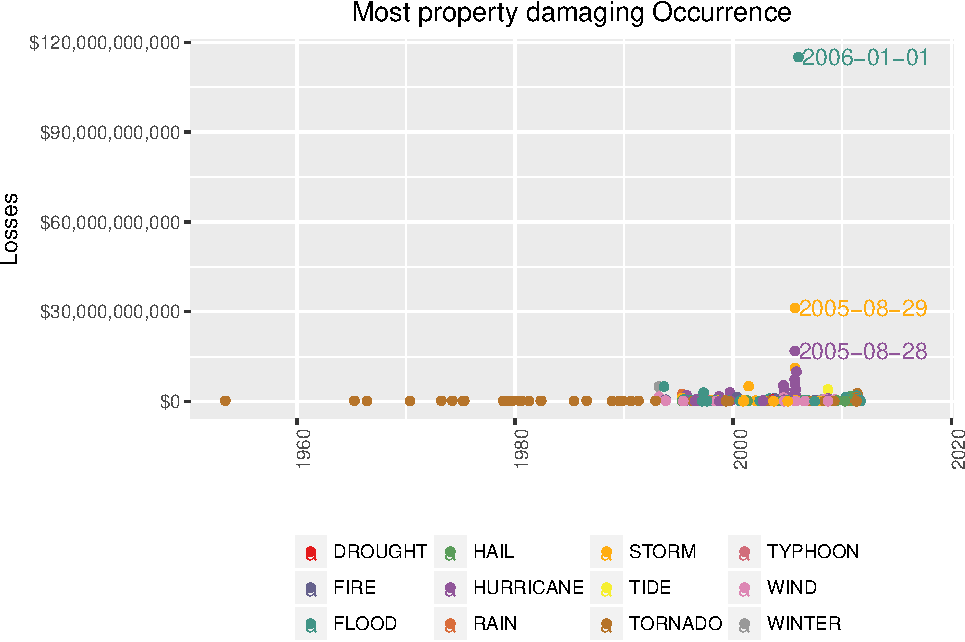
\includegraphics{readme_files/figure-latex/prop-single-plot-1.pdf}

The single most economic damaging event to properties was a
\textbf{FLOOD, that occurred in CA, NAPA, on 2006-01-01, causing U\$
\$115,000,000,000 in losses}.

\subsection{Most Property Damaging event in all
time}\label{most-property-damaging-event-in-all-time}

Most Property Damaging event in all time

Notice that are several occurrences of the same type of event along the
time.

Therefore, in order to know which is the worst type of event along all
the years, we summed up the losses caused by each one of occurrences of
this events.

Notice that we are interested only in the worst of them, ie, the ones
which are above the mean.

\begin{Shaded}
\begin{Highlighting}[]
\CommentTok{# totals per event}
\NormalTok{prop.all.df <-}\StringTok{ }\NormalTok{prop.df %>%}\StringTok{ }\KeywordTok{group_by}\NormalTok{(event) %>%}
\StringTok{                }\KeywordTok{summarise}\NormalTok{(}\DataTypeTok{total.raw =} \KeywordTok{sum}\NormalTok{(prop.ev)) %>%}
\StringTok{                }\KeywordTok{arrange}\NormalTok{(}\KeywordTok{desc}\NormalTok{(total.raw)) %>%}
\StringTok{                }\KeywordTok{mutate}\NormalTok{(}\DataTypeTok{media.raw =} \KeywordTok{mean}\NormalTok{(total.raw), }
                        \DataTypeTok{mediana.raw =} \KeywordTok{median}\NormalTok{(total.raw),}
                        \DataTypeTok{total =} \KeywordTok{dollar}\NormalTok{(total.raw),}
                        \DataTypeTok{mean =} \KeywordTok{dollar}\NormalTok{(media.raw),}
                        \DataTypeTok{median =} \KeywordTok{dollar}\NormalTok{(mediana.raw),}
                        \DataTypeTok{rank =} \KeywordTok{seq_len}\NormalTok{(}\KeywordTok{length}\NormalTok{(event))) %>%}
\StringTok{                }\KeywordTok{filter}\NormalTok{(total.raw >}\StringTok{ }\KeywordTok{mean}\NormalTok{(total.raw))}
                
\CommentTok{# create color pallete for all events}
\NormalTok{colourCount.prop.all =}\StringTok{ }\KeywordTok{length}\NormalTok{(}\KeywordTok{unique}\NormalTok{(prop.all.df$event))}
\NormalTok{getPalette =}\StringTok{ }\KeywordTok{colorRampPalette}\NormalTok{(}\KeywordTok{brewer.pal}\NormalTok{(colourCount.prop.all, }\StringTok{"Set1"}\NormalTok{))}

\CommentTok{# prepare text for inline R}
\NormalTok{worst.prop.all.ev <-}\StringTok{ }\NormalTok{prop.all.df$event[}\DecValTok{1}\NormalTok{]}
\NormalTok{worst.prop.total <-}\StringTok{ }\NormalTok{prop.all.df$total[}\DecValTok{1}\NormalTok{]}

\CommentTok{# a table}
\KeywordTok{kable}\NormalTok{(prop.all.df[, }\KeywordTok{c}\NormalTok{(}\DecValTok{8}\NormalTok{,}\DecValTok{1}\NormalTok{,}\DecValTok{5}\NormalTok{:}\DecValTok{7}\NormalTok{)])}
\end{Highlighting}
\end{Shaded}

\begin{longtable}[]{@{}rllll@{}}
\toprule
rank & event & total & mean & median\tabularnewline
\midrule
\endhead
1 & FLOOD & \$168,258,894,238 & \$9,309,236,205 &
\$6,537,750\tabularnewline
2 & HURRICANE & \$84,656,180,010 & \$9,309,236,205 &
\$6,537,750\tabularnewline
3 & TORNADO & \$57,003,317,814 & \$9,309,236,205 &
\$6,537,750\tabularnewline
4 & STORM & \$56,197,366,960 & \$9,309,236,205 &
\$6,537,750\tabularnewline
5 & WIND & \$17,951,211,793 & \$9,309,236,205 &
\$6,537,750\tabularnewline
6 & HAIL & \$15,977,047,956 & \$9,309,236,205 &
\$6,537,750\tabularnewline
\bottomrule
\end{longtable}

\begin{Shaded}
\begin{Highlighting}[]
\NormalTok{plt.prop.all <-}\StringTok{ }\KeywordTok{ggplot}\NormalTok{(}\DataTypeTok{data=}\NormalTok{prop.all.df, }\KeywordTok{aes}\NormalTok{(event, total.raw, }\DataTypeTok{fill=}\NormalTok{event))}

\NormalTok{plt.prop.all <-}\StringTok{ }\NormalTok{plt.prop.all +}\StringTok{ }\KeywordTok{geom_bar}\NormalTok{(}\DataTypeTok{stat=}\StringTok{"identity"}\NormalTok{) +}
\StringTok{                }
\StringTok{        }\KeywordTok{geom_text}\NormalTok{(}\KeywordTok{aes}\NormalTok{(}\DataTypeTok{label=}\KeywordTok{ifelse}\NormalTok{(total.raw==}\KeywordTok{max}\NormalTok{(total.raw),}
                \KeywordTok{paste}\NormalTok{(event, }\KeywordTok{dollar}\NormalTok{(}\KeywordTok{max}\NormalTok{(total.raw)), }\DataTypeTok{sep=}\StringTok{": "}\NormalTok{),}\StringTok{''}\NormalTok{)),}
                \DataTypeTok{hjust=}\DecValTok{0}\NormalTok{,}\DataTypeTok{vjust=}\DecValTok{2}\NormalTok{) +}
\StringTok{        }\KeywordTok{geom_hline}\NormalTok{(}\KeywordTok{aes}\NormalTok{(}\DataTypeTok{yintercept =} \NormalTok{media.raw), }\DataTypeTok{linetype=}\DecValTok{1}\NormalTok{) +}
\StringTok{        }\CommentTok{# geom_hline(aes(yintercept = mediana.raw), linetype=2) +}
\StringTok{        }\KeywordTok{labs}\NormalTok{(}\DataTypeTok{title=}\StringTok{"All time"}\NormalTok{, }\DataTypeTok{y=}\StringTok{""}\NormalTok{, }\DataTypeTok{x=}\StringTok{""}\NormalTok{) +}\StringTok{ }
\StringTok{                }
\StringTok{        }\KeywordTok{scale_y_continuous}\NormalTok{(}\DataTypeTok{labels =} \NormalTok{dollar)+}
\StringTok{     }
\StringTok{        }\KeywordTok{theme}\NormalTok{(}\DataTypeTok{legend.position=}\StringTok{"none"}\NormalTok{) +}\StringTok{        }
\StringTok{        }\KeywordTok{scale_colour_manual}\NormalTok{(}\DataTypeTok{values =} \KeywordTok{getPalette}\NormalTok{(colourCount.prop.all))+}\StringTok{                }
\StringTok{        }\KeywordTok{theme}\NormalTok{(}\DataTypeTok{legend.title=}\KeywordTok{element_blank}\NormalTok{()) +}
\StringTok{        }\KeywordTok{theme}\NormalTok{(}\DataTypeTok{axis.text.x =} \KeywordTok{element_text}\NormalTok{(}\DataTypeTok{angle =} \DecValTok{90}\NormalTok{, }\DataTypeTok{hjust =} \DecValTok{1}\NormalTok{)) +}\StringTok{ }
\StringTok{        }\KeywordTok{theme}\NormalTok{(}\DataTypeTok{plot.title =} \KeywordTok{element_text}\NormalTok{(}\DataTypeTok{hjust =} \FloatTok{0.5}\NormalTok{))                 }

\NormalTok{plt.prop.all +}\StringTok{ }\KeywordTok{labs}\NormalTok{(}\DataTypeTok{title=}\StringTok{"Most property damaging type of event - all time"}\NormalTok{,}
                    \DataTypeTok{y=}\StringTok{"Losses"}\NormalTok{, }\DataTypeTok{x=}\StringTok{""}\NormalTok{)}
\end{Highlighting}
\end{Shaded}

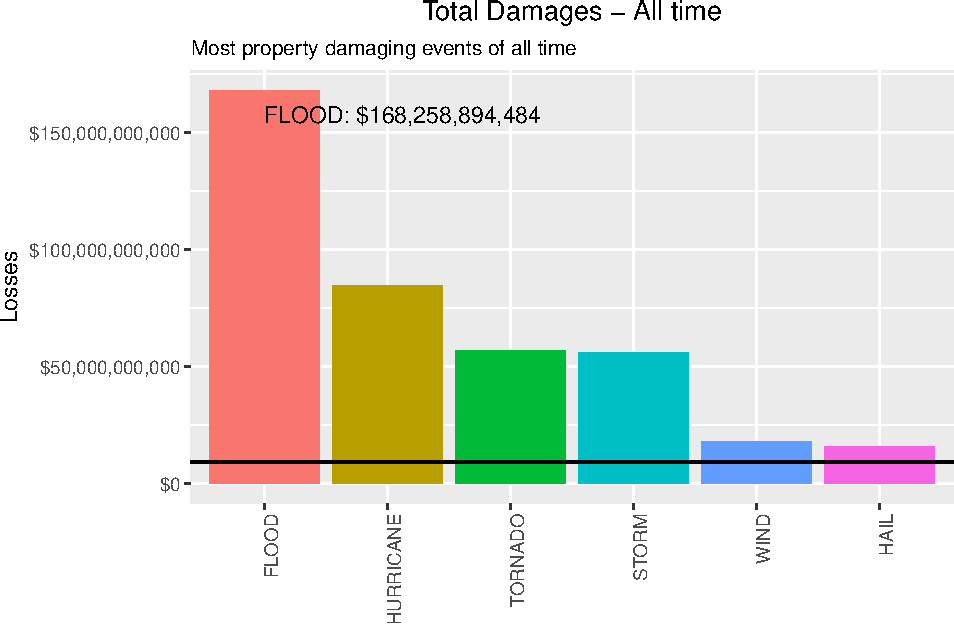
\includegraphics{readme_files/figure-latex/prop-all-plot-1.pdf}

The most property damaging event along the time is the \textbf{FLOOD. It
has caused \$168,258,894,238 in losses.}

Just for curiosity, these are the less damaging events:

\begin{Shaded}
\begin{Highlighting}[]
\NormalTok{prop.all.df <-}\StringTok{ }\NormalTok{prop.df %>%}\StringTok{ }\KeywordTok{group_by}\NormalTok{(event) %>%}
\StringTok{                }\KeywordTok{summarise}\NormalTok{(}\DataTypeTok{total.raw =} \KeywordTok{sum}\NormalTok{(prop.ev)) %>%}
\StringTok{                }\KeywordTok{arrange}\NormalTok{(total.raw) %>%}
\StringTok{                }\KeywordTok{mutate}\NormalTok{(}\DataTypeTok{media.raw =} \KeywordTok{mean}\NormalTok{(total.raw), }
                        \DataTypeTok{mediana.raw =} \KeywordTok{median}\NormalTok{(total.raw),}
                        \DataTypeTok{total =} \KeywordTok{dollar}\NormalTok{(total.raw),}
                        \DataTypeTok{mean =} \KeywordTok{dollar}\NormalTok{(media.raw),}
                        \DataTypeTok{median =} \KeywordTok{dollar}\NormalTok{(mediana.raw),}
                        \DataTypeTok{rank =} \KeywordTok{seq}\NormalTok{(}\KeywordTok{length}\NormalTok{(event),}\DecValTok{1}\NormalTok{, }\DataTypeTok{by=}\NormalTok{-}\DecValTok{1}\NormalTok{))}



\KeywordTok{kable}\NormalTok{(prop.all.df[}\DecValTok{1}\NormalTok{:}\DecValTok{10}\NormalTok{, }\KeywordTok{c}\NormalTok{(}\DecValTok{8}\NormalTok{,}\DecValTok{1}\NormalTok{,}\DecValTok{5}\NormalTok{:}\DecValTok{7}\NormalTok{)])}
\end{Highlighting}
\end{Shaded}

\begin{longtable}[]{@{}rllll@{}}
\toprule
rank & event & total & mean & median\tabularnewline
\midrule
\endhead
46 & RIP CURRENT & \$1,000 & \$9,309,236,205 &
\$6,537,750\tabularnewline
45 & HIGH SWELLS & \$5,000 & \$9,309,236,205 &
\$6,537,750\tabularnewline
44 & URBAN/SMALL STREAM & \$5,000 & \$9,309,236,205 &
\$6,537,750\tabularnewline
43 & WINTRY MIX & \$12,500 & \$9,309,236,205 &
\$6,537,750\tabularnewline
42 & FROST & \$15,000 & \$9,309,236,205 & \$6,537,750\tabularnewline
41 & HIGH SEAS & \$15,500 & \$9,309,236,205 & \$6,537,750\tabularnewline
40 & WET MICROBURST & \$35,000 & \$9,309,236,205 &
\$6,537,750\tabularnewline
39 & MICROBURST & \$80,000 & \$9,309,236,205 &
\$6,537,750\tabularnewline
38 & DENSE SMOKE & \$100,000 & \$9,309,236,205 &
\$6,537,750\tabularnewline
37 & GUSTNADO & \$102,050 & \$9,309,236,205 & \$6,537,750\tabularnewline
\bottomrule
\end{longtable}

\subsection{Crop losses}\label{crop-losses}

\subsection{Most Crop Damaging event in a single
occurrence}\label{most-crop-damaging-event-in-a-single-occurrence}

Most Crop Damaging event in a single occurrence

In order to determine what were the most crop damaging events in a
single occurrence, we need to see how damages are distributed along the
occurrences.

\begin{Shaded}
\begin{Highlighting}[]
\CommentTok{# crop damages}
\KeywordTok{rm}\NormalTok{(prop.df, prop.all.df, prop95.df) }\CommentTok{# cleannig house}

\NormalTok{crop.df <-}\StringTok{ }\NormalTok{harm.df %>%}\StringTok{ }\KeywordTok{filter}\NormalTok{(!}\KeywordTok{is.na}\NormalTok{(crop.ev)) %>%}
\StringTok{                }\KeywordTok{select}\NormalTok{(}\DecValTok{1}\NormalTok{:}\DecValTok{6}\NormalTok{,}\DecValTok{14}\NormalTok{) }


\CommentTok{# quantiles}
\NormalTok{qt <-}\StringTok{ }\KeywordTok{quantile}\NormalTok{(crop.df$crop.ev, }\DataTypeTok{probs=}\KeywordTok{seq}\NormalTok{(.}\DecValTok{998}\NormalTok{,}\DecValTok{1}\NormalTok{,}\FloatTok{0.002}\NormalTok{))}

\CommentTok{# distribution plot}
\NormalTok{plt.distr.crop0 <-}\StringTok{ }\KeywordTok{ggplot}\NormalTok{(crop.df, }\KeywordTok{aes}\NormalTok{(}\KeywordTok{log}\NormalTok{(crop.ev)))}

\NormalTok{plt.distr.crop0 <-}\StringTok{ }\NormalTok{plt.distr.crop0 +}\StringTok{ }\KeywordTok{geom_density}\NormalTok{(}\KeywordTok{aes}\NormalTok{(}\DataTypeTok{y=}\NormalTok{..density..)) +}\StringTok{ }\CommentTok{#xlim(0,.5) + }
\StringTok{        }\KeywordTok{labs}\NormalTok{(}\DataTypeTok{title=}\StringTok{"All events"}\NormalTok{, }\DataTypeTok{x=}\StringTok{"log(amount $)"}\NormalTok{) +}
\StringTok{        }\KeywordTok{theme}\NormalTok{(}\DataTypeTok{plot.title =} \KeywordTok{element_text}\NormalTok{(}\DataTypeTok{hjust =} \FloatTok{0.5}\NormalTok{))  }


\CommentTok{# display only the qts next to harmfull events}
\NormalTok{qt}
\end{Highlighting}
\end{Shaded}

\begin{verbatim}
##      99.8%       100% 
##    7000000 5000000000
\end{verbatim}

Looking at this distribution, we can infer that 99\% of the occurrences
caused less than \textbf{\$7,000,000 in losses}.

On the other hand, damaging occurrences had to have damages above zero.

Now, among the damaging occurrences, we are interested in the ones whose
damages are above 99\% of the most common values.

\begin{Shaded}
\begin{Highlighting}[]
\CommentTok{# subset for harm events}
\NormalTok{crop.df <-}\StringTok{ }\NormalTok{crop.df %>%}\StringTok{ }\KeywordTok{filter}\NormalTok{(crop.ev >}\StringTok{ }\DecValTok{0}\NormalTok{) %>%}
\StringTok{                }\KeywordTok{arrange}\NormalTok{(}\KeywordTok{desc}\NormalTok{(crop.ev)) %>%}
\StringTok{                }\KeywordTok{mutate}\NormalTok{(}\DataTypeTok{value =} \KeywordTok{dollar}\NormalTok{(crop.ev),}
                        \DataTypeTok{media.raw =} \KeywordTok{mean}\NormalTok{(crop.ev), }
                        \DataTypeTok{mediana.raw =} \KeywordTok{median}\NormalTok{(crop.ev),}
                        \DataTypeTok{mean =} \KeywordTok{dollar}\NormalTok{(media.raw),}
                        \DataTypeTok{median =} \KeywordTok{dollar}\NormalTok{(mediana.raw),}
                        \DataTypeTok{rank =} \KeywordTok{seq_len}\NormalTok{(}\KeywordTok{length}\NormalTok{(event)))}

\CommentTok{# quantiles, same as }
\CommentTok{# poisson.test(mean, conf.level = 0.95)}

\NormalTok{qt <-}\StringTok{ }\KeywordTok{quantile}\NormalTok{(crop.df$crop.ev, }\DataTypeTok{probs=}\KeywordTok{seq}\NormalTok{(.}\DecValTok{999}\NormalTok{,}\DecValTok{1}\NormalTok{,}\FloatTok{0.005}\NormalTok{))}
\NormalTok{qt}
\end{Highlighting}
\end{Shaded}

\begin{verbatim}
##     99.9% 
## 336111520
\end{verbatim}

Looking at this distribution, we can infer that \textbf{99.8\% of the
damaging occurrences caused up to \$336,111,520 in losses.}

Distribution plots

\begin{Shaded}
\begin{Highlighting}[]
\CommentTok{# distribution plot}
\NormalTok{plt.distr.crop1 <-}\StringTok{ }\KeywordTok{ggplot}\NormalTok{(crop.df, }\KeywordTok{aes}\NormalTok{(}\KeywordTok{log}\NormalTok{(crop.ev)))}

\NormalTok{plt.distr.crop1 <-}\StringTok{ }\NormalTok{plt.distr.crop1 +}\StringTok{ }\KeywordTok{geom_density}\NormalTok{(}\KeywordTok{aes}\NormalTok{(}\DataTypeTok{y=}\NormalTok{..density..)) +}\StringTok{ }\CommentTok{#xlim(0,qt[1]) + }
\StringTok{        }\KeywordTok{labs}\NormalTok{(}\DataTypeTok{title=}\StringTok{"Damaging events"}\NormalTok{, }\DataTypeTok{x=}\StringTok{"log(amount $)"}\NormalTok{) +}
\StringTok{        }\CommentTok{# scale_x_continuous(labels = dollar)+}
\StringTok{        }\CommentTok{# theme(axis.text.x = element_text(angle = 90, hjust = 1)) + }
\StringTok{        }\KeywordTok{theme}\NormalTok{(}\DataTypeTok{plot.title =} \KeywordTok{element_text}\NormalTok{(}\DataTypeTok{hjust =} \FloatTok{0.5}\NormalTok{))       }
\end{Highlighting}
\end{Shaded}

\begin{Shaded}
\begin{Highlighting}[]
\KeywordTok{grid.arrange}\NormalTok{(plt.distr.crop0, plt.distr.crop1,}
             \DataTypeTok{nrow=}\DecValTok{1}\NormalTok{, }\DataTypeTok{ncol=}\DecValTok{2}\NormalTok{, }
             \DataTypeTok{bottom=}\StringTok{"Population distribution"}\NormalTok{)}
\KeywordTok{grid.rect}\NormalTok{(}\DataTypeTok{gp=}\KeywordTok{gpar}\NormalTok{(}\DataTypeTok{fill=}\OtherTok{NA}\NormalTok{))}
\end{Highlighting}
\end{Shaded}

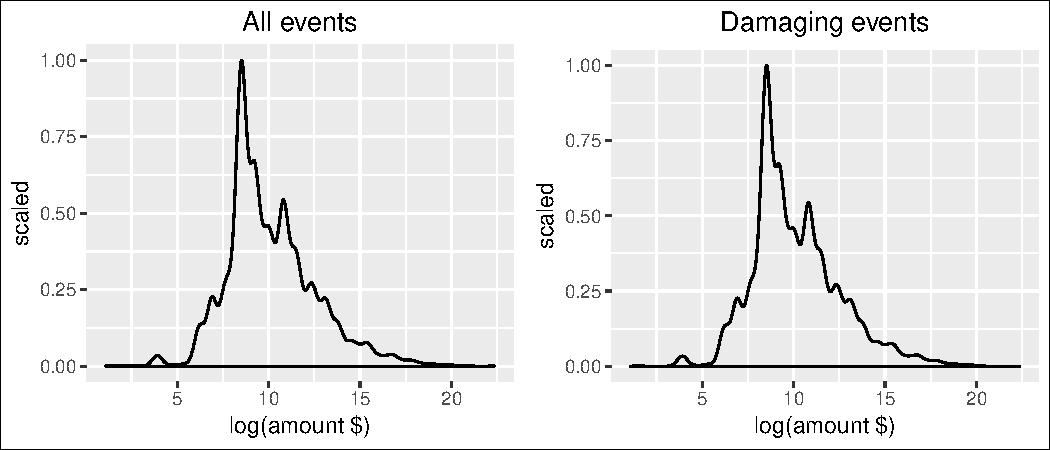
\includegraphics{readme_files/figure-latex/crop-distr-4-1.pdf}

In this study, we looked on the 1\% most harmful occurrences.

\begin{Shaded}
\begin{Highlighting}[]
\CommentTok{# subset for 99% CI}
\NormalTok{crop95.df <-}\StringTok{ }\KeywordTok{filter}\NormalTok{(crop.df, crop.ev>qt[}\DecValTok{1}\NormalTok{])}

\CommentTok{# create color pallete for all events}
\NormalTok{colourCount.crop.single =}\StringTok{ }\KeywordTok{length}\NormalTok{(}\KeywordTok{unique}\NormalTok{(crop95.df$event))}
\NormalTok{getPalette =}\StringTok{ }\KeywordTok{colorRampPalette}\NormalTok{(}\KeywordTok{brewer.pal}\NormalTok{(colourCount.crop.single, }\StringTok{"Set1"}\NormalTok{))}


\CommentTok{# print a table}
\KeywordTok{kable}\NormalTok{(crop95.df[}\DecValTok{1}\NormalTok{:}\DecValTok{20}\NormalTok{,}\KeywordTok{c}\NormalTok{(}\DecValTok{13}\NormalTok{,}\DecValTok{1}\NormalTok{:}\DecValTok{6}\NormalTok{,}\DecValTok{8}\NormalTok{,}\DecValTok{11}\NormalTok{:}\DecValTok{12}\NormalTok{)])}
\end{Highlighting}
\end{Shaded}

\begin{longtable}[]{@{}rlrlrlllll@{}}
\toprule
rank & event & mag & day & duration & state & countyname & value & mean
& median\tabularnewline
\midrule
\endhead
1 & FLOOD & 0 & 1993-08-31 & NA & IL & ADAMS & \$5,000,000,000 &
\$2,224,406 & \$15,000\tabularnewline
2 & STORM & 0 & 1994-02-09 & 0S & MS & MSZ001 & \$5,000,000,000 &
\$2,224,406 & \$15,000\tabularnewline
3 & HURRICANE & 0 & 2005-08-29 & 0S & MS & MSZ018 & \$1,510,000,000 &
\$2,224,406 & \$15,000\tabularnewline
4 & DROUGHT & 0 & 2006-01-01 & 0S & TX & TXZ091 & \$1,000,000,000 &
\$2,224,406 & \$15,000\tabularnewline
5 & COLD & 0 & 1998-12-20 & 0S & CA & CAZ020 & \$596,000,000 &
\$2,224,406 & \$15,000\tabularnewline
6 & DROUGHT & 0 & 2001-08-01 & 0S & IA & IAZ004 & \$578,850,000 &
\$2,224,406 & \$15,000\tabularnewline
7 & DROUGHT & 0 & 2000-11-01 & 0S & TX & TXZ021 & \$515,000,000 &
\$2,224,406 & \$15,000\tabularnewline
8 & DROUGHT & 0 & 1995-08-01 & 0S & IA & IAZ004 & \$500,000,000 &
\$2,224,406 & \$15,000\tabularnewline
9 & DROUGHT & 0 & 1998-07-06 & 0S & OK & OKZ049 & \$500,000,000 &
\$2,224,406 & \$15,000\tabularnewline
10 & HURRICANE & 0 & 1999-09-15 & 0S & NC & NCZ007 & \$500,000,000 &
\$2,224,406 & \$15,000\tabularnewline
11 & DROUGHT & 0 & 1999-07-01 & 0S & PA & PAZ006 & \$500,000,000 &
\$2,224,406 & \$15,000\tabularnewline
12 & FLOOD & 0 & 2000-10-03 & 0S & FL & FLZ072 & \$500,000,000 &
\$2,224,406 & \$15,000\tabularnewline
13 & FLOOD & 0 & 2007-07-01 & 0S & MO & HENRY & \$500,000,000 &
\$2,224,406 & \$15,000\tabularnewline
14 & HEAT & 0 & 2006-07-16 & 0S & CA & CAZ089 & \$492,400,000 &
\$2,224,406 & \$15,000\tabularnewline
15 & DROUGHT & 0 & 2002-12-01 & 0S & NE & NEZ039 & \$480,000,000 &
\$2,224,406 & \$15,000\tabularnewline
16 & DROUGHT & 0 & 1998-12-01 & 0S & TX & TXZ021 & \$450,000,000 &
\$2,224,406 & \$15,000\tabularnewline
17 & HURRICANE & 0 & 2005-08-25 & 0S & FL & FLZ068 & \$423,000,000 &
\$2,224,406 & \$15,000\tabularnewline
18 & DROUGHT & 0 & 2001-12-01 & 0S & TX & TXZ021 & \$420,000,000 &
\$2,224,406 & \$15,000\tabularnewline
19 & HURRICANE & 0 & 1999-09-14 & 0S & NC & NCZ029 & \$413,600,000 &
\$2,224,406 & \$15,000\tabularnewline
20 & HEAT & 0 & 1995-08-20 & NA & AL & TALLADEGA & \$400,000,000 &
\$2,224,406 & \$15,000\tabularnewline
\bottomrule
\end{longtable}

\begin{Shaded}
\begin{Highlighting}[]
\NormalTok{worst.crop.single.ev <-}\StringTok{ }\NormalTok{crop95.df$event[}\DecValTok{1}\NormalTok{]}
\NormalTok{worst.crop.single.st <-}\StringTok{ }\NormalTok{crop95.df$state[}\DecValTok{1}\NormalTok{]}
\NormalTok{worst.crop.single.ct <-}\StringTok{ }\NormalTok{crop95.df$countyname[}\DecValTok{1}\NormalTok{]}
\NormalTok{worst.crop.single.dt <-}\StringTok{ }\NormalTok{crop95.df$day[}\DecValTok{1}\NormalTok{]}
\NormalTok{worst.crop.single.value <-}\StringTok{ }\NormalTok{crop95.df$value[}\DecValTok{1}\NormalTok{]}
\end{Highlighting}
\end{Shaded}

\begin{Shaded}
\begin{Highlighting}[]
\NormalTok{plt.crop.single <-}\StringTok{ }\KeywordTok{ggplot}\NormalTok{(crop95.df, }\KeywordTok{aes}\NormalTok{(day, crop.ev, }\DataTypeTok{colour=}\NormalTok{event))}

\NormalTok{plt.crop.single <-}\StringTok{ }\NormalTok{plt.crop.single +}\StringTok{ }\KeywordTok{geom_point}\NormalTok{() +}
\StringTok{        }\KeywordTok{geom_text}\NormalTok{(}\KeywordTok{aes}\NormalTok{(}\DataTypeTok{label=}\KeywordTok{ifelse}\NormalTok{(rank <=}\StringTok{ }\DecValTok{3}\NormalTok{,}
                \KeywordTok{as.character}\NormalTok{(day),}\StringTok{""}\NormalTok{),}
                \DataTypeTok{hjust=}\NormalTok{-.}\DecValTok{03}\NormalTok{,}\DataTypeTok{vjust=}\FloatTok{0.5}\NormalTok{)) +}
\StringTok{        }\CommentTok{# geom_hline(aes(yintercept = media.raw), linetype=2) +}
\StringTok{        }\CommentTok{# geom_hline(aes(yintercept = mediana.raw), linetype=3) +}
\StringTok{        }\KeywordTok{labs}\NormalTok{(}\DataTypeTok{title=}\StringTok{"Crop Dammaging"}\NormalTok{,}
                    \DataTypeTok{y=}\StringTok{""}\NormalTok{, }\DataTypeTok{x=}\StringTok{""}\NormalTok{) +}\StringTok{ }
\StringTok{                }
\StringTok{        }\KeywordTok{expand_limits}\NormalTok{(}\DataTypeTok{x=}\KeywordTok{as.Date}\NormalTok{(}\StringTok{'2017-01-01'}\NormalTok{))+}\StringTok{ }\CommentTok{#ok}
\StringTok{        }\KeywordTok{scale_y_continuous}\NormalTok{(}\DataTypeTok{labels =} \NormalTok{dollar)+}
\StringTok{        }
\StringTok{        }\KeywordTok{scale_colour_manual}\NormalTok{(}\DataTypeTok{values =} \KeywordTok{getPalette}\NormalTok{(colourCount.crop.single))+}\StringTok{                }
\StringTok{        }\KeywordTok{theme}\NormalTok{(}\DataTypeTok{legend.title=}\KeywordTok{element_blank}\NormalTok{()) +}
\StringTok{        }\KeywordTok{theme}\NormalTok{(}\DataTypeTok{legend.position=}\StringTok{"bottom"}\NormalTok{) +}
\StringTok{        }\KeywordTok{guides}\NormalTok{(}\DataTypeTok{fill=}\KeywordTok{guide_legend}\NormalTok{(}\DataTypeTok{nrow=}\DecValTok{5}\NormalTok{, }\DataTypeTok{byrow=}\OtherTok{TRUE}\NormalTok{)) +}
\StringTok{        }\KeywordTok{theme}\NormalTok{(}\DataTypeTok{axis.text.x =} \KeywordTok{element_text}\NormalTok{(}\DataTypeTok{angle =} \DecValTok{90}\NormalTok{, }\DataTypeTok{hjust =} \DecValTok{1}\NormalTok{)) +}\StringTok{ }
\StringTok{        }\KeywordTok{theme}\NormalTok{(}\DataTypeTok{plot.title =} \KeywordTok{element_text}\NormalTok{(}\DataTypeTok{hjust =} \FloatTok{0.5}\NormalTok{)) }

\NormalTok{plt.crop.single +}\StringTok{ }\KeywordTok{labs}\NormalTok{(}\DataTypeTok{title=}\StringTok{"Most crop damaging Occurrence"}\NormalTok{,}
                    \DataTypeTok{y=}\StringTok{"Losses"}\NormalTok{, }\DataTypeTok{x=}\StringTok{""}\NormalTok{)}
\end{Highlighting}
\end{Shaded}

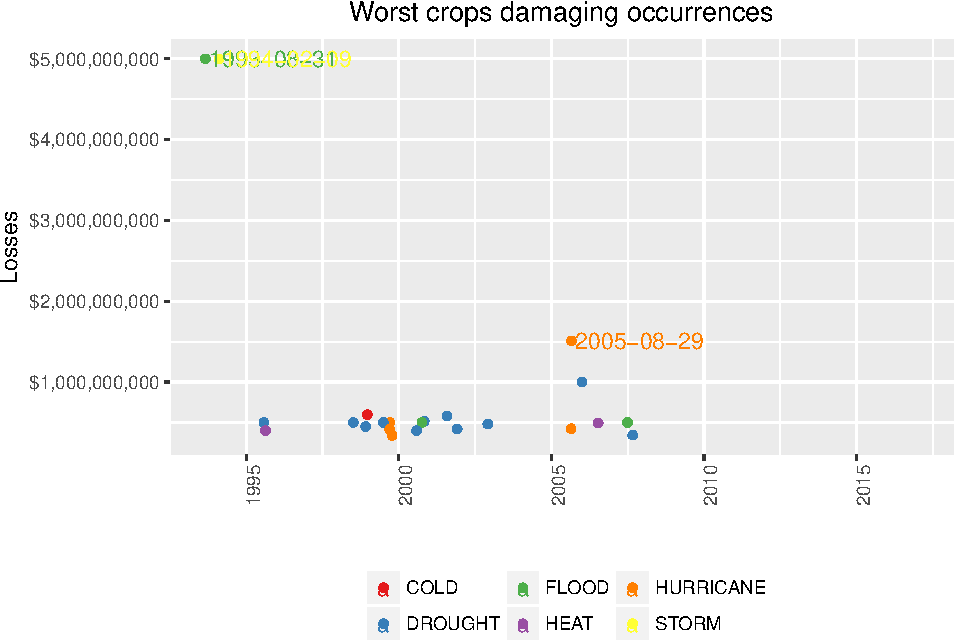
\includegraphics{readme_files/figure-latex/crop-single-plot-1.pdf}

The single most economic damaging event to crops was a \textbf{FLOOD,
that occurred in IL, ADAMS, on 1993-08-31, causing U\$ \$5,000,000,000
in losses.}

\subsection{Most Crop Damaging event in all
time}\label{most-crop-damaging-event-in-all-time}

Most Crop Damaging event in all time

Notice that are several occurrences of the same type of event along the
time.

Therefore, in order to know which is the worst type of event along all
the years, we summed up the losses caused by each one of occurrences of
this events.

Notice that we are interested only in the worst of them, ie, the ones
which are above the mean.

\begin{Shaded}
\begin{Highlighting}[]
\CommentTok{# totals per event}
\NormalTok{crop.all.df <-}\StringTok{ }\NormalTok{crop.df %>%}\StringTok{ }\KeywordTok{group_by}\NormalTok{(event) %>%}
\StringTok{                }\KeywordTok{summarise}\NormalTok{(}\DataTypeTok{total.raw =} \KeywordTok{sum}\NormalTok{(crop.ev)) %>%}
\StringTok{                }\KeywordTok{arrange}\NormalTok{(}\KeywordTok{desc}\NormalTok{(total.raw)) %>%}
\StringTok{                }\KeywordTok{mutate}\NormalTok{(}\DataTypeTok{media.raw =} \KeywordTok{mean}\NormalTok{(total.raw), }
                        \DataTypeTok{mediana.raw =} \KeywordTok{median}\NormalTok{(total.raw),}
                        \DataTypeTok{total =} \KeywordTok{dollar}\NormalTok{(total.raw),}
                        \DataTypeTok{mean =} \KeywordTok{dollar}\NormalTok{(media.raw),}
                        \DataTypeTok{median =} \KeywordTok{dollar}\NormalTok{(mediana.raw),}
                        \DataTypeTok{rank =} \KeywordTok{seq_len}\NormalTok{(}\KeywordTok{length}\NormalTok{(event))) %>%}
\StringTok{                }\KeywordTok{filter}\NormalTok{(total.raw >}\StringTok{ }\KeywordTok{mean}\NormalTok{(total.raw))}
                
\CommentTok{# create color pallete for all events}
\NormalTok{colourCount.crop.all =}\StringTok{ }\KeywordTok{length}\NormalTok{(}\KeywordTok{unique}\NormalTok{(crop.all.df$event))}
\NormalTok{getPalette =}\StringTok{ }\KeywordTok{colorRampPalette}\NormalTok{(}\KeywordTok{brewer.pal}\NormalTok{(colourCount.crop.all, }\StringTok{"Set1"}\NormalTok{))}

\CommentTok{# prepare text for inline R}
\NormalTok{worst.crop.all.ev <-}\StringTok{ }\NormalTok{crop.all.df$event[}\DecValTok{1}\NormalTok{]}
\NormalTok{worst.crop.total <-}\StringTok{ }\NormalTok{crop.all.df$total[}\DecValTok{1}\NormalTok{]}

\CommentTok{# a table}
\KeywordTok{kable}\NormalTok{(crop.all.df[, }\KeywordTok{c}\NormalTok{(}\DecValTok{8}\NormalTok{,}\DecValTok{1}\NormalTok{,}\DecValTok{5}\NormalTok{:}\DecValTok{7}\NormalTok{)])}
\end{Highlighting}
\end{Shaded}

\begin{longtable}[]{@{}rllll@{}}
\toprule
rank & event & total & mean & median\tabularnewline
\midrule
\endhead
1 & DROUGHT & \$13,972,581,000 & \$2,231,988,917 &
\$296,658,415\tabularnewline
2 & FLOOD & \$12,275,737,200 & \$2,231,988,917 &
\$296,658,415\tabularnewline
3 & STORM & \$5,738,319,500 & \$2,231,988,917 &
\$296,658,415\tabularnewline
4 & HURRICANE & \$5,505,292,800 & \$2,231,988,917 &
\$296,658,415\tabularnewline
5 & COLD & \$3,298,176,550 & \$2,231,988,917 &
\$296,658,415\tabularnewline
6 & HAIL & \$3,046,470,470 & \$2,231,988,917 &
\$296,658,415\tabularnewline
\bottomrule
\end{longtable}

\begin{Shaded}
\begin{Highlighting}[]
\NormalTok{plt.crop.all <-}\StringTok{ }\KeywordTok{ggplot}\NormalTok{(}\DataTypeTok{data=}\NormalTok{crop.all.df, }\KeywordTok{aes}\NormalTok{(event, total.raw, }\DataTypeTok{fill=}\NormalTok{event))}

\NormalTok{plt.crop.all <-}\StringTok{ }\NormalTok{plt.crop.all +}\StringTok{ }\KeywordTok{geom_bar}\NormalTok{(}\DataTypeTok{stat=}\StringTok{"identity"}\NormalTok{) +}
\StringTok{                }
\StringTok{        }\KeywordTok{geom_text}\NormalTok{(}\KeywordTok{aes}\NormalTok{(}\DataTypeTok{label=}\KeywordTok{ifelse}\NormalTok{(total.raw==}\KeywordTok{max}\NormalTok{(total.raw),}
                \KeywordTok{paste}\NormalTok{(event, }\KeywordTok{dollar}\NormalTok{(}\KeywordTok{max}\NormalTok{(total.raw)), }\DataTypeTok{sep=}\StringTok{": "}\NormalTok{),}\StringTok{''}\NormalTok{)),}
                \DataTypeTok{hjust=}\DecValTok{0}\NormalTok{,}\DataTypeTok{vjust=}\DecValTok{2}\NormalTok{) +}
\StringTok{        }\KeywordTok{geom_hline}\NormalTok{(}\KeywordTok{aes}\NormalTok{(}\DataTypeTok{yintercept =} \NormalTok{media.raw), }\DataTypeTok{linetype=}\DecValTok{1}\NormalTok{) +}
\StringTok{        }\CommentTok{# geom_hline(aes(yintercept = mediana.raw), linetype=2) +}
\StringTok{        }\KeywordTok{labs}\NormalTok{(}\DataTypeTok{title=}\StringTok{"All time"}\NormalTok{, }\DataTypeTok{y=}\StringTok{""}\NormalTok{, }\DataTypeTok{x=}\StringTok{""}\NormalTok{) +}\StringTok{ }
\StringTok{                }
\StringTok{        }\KeywordTok{scale_y_continuous}\NormalTok{(}\DataTypeTok{labels =} \NormalTok{dollar)+}
\StringTok{     }
\StringTok{        }\KeywordTok{theme}\NormalTok{(}\DataTypeTok{legend.position=}\StringTok{"none"}\NormalTok{) +}\StringTok{        }
\StringTok{        }\KeywordTok{scale_colour_manual}\NormalTok{(}\DataTypeTok{values =} \KeywordTok{getPalette}\NormalTok{(colourCount.crop.all))+}\StringTok{                }
\StringTok{        }\KeywordTok{theme}\NormalTok{(}\DataTypeTok{legend.title=}\KeywordTok{element_blank}\NormalTok{()) +}
\StringTok{        }\KeywordTok{theme}\NormalTok{(}\DataTypeTok{axis.text.x =} \KeywordTok{element_text}\NormalTok{(}\DataTypeTok{angle =} \DecValTok{90}\NormalTok{, }\DataTypeTok{hjust =} \DecValTok{1}\NormalTok{)) +}\StringTok{ }
\StringTok{        }\KeywordTok{theme}\NormalTok{(}\DataTypeTok{plot.title =} \KeywordTok{element_text}\NormalTok{(}\DataTypeTok{hjust =} \FloatTok{0.5}\NormalTok{))                 }

\NormalTok{plt.crop.all +}\StringTok{ }\KeywordTok{labs}\NormalTok{(}\DataTypeTok{title=}\StringTok{"Most crops damaging type of event - all time"}\NormalTok{,}
                    \DataTypeTok{y=}\StringTok{"Losses"}\NormalTok{, }\DataTypeTok{x=}\StringTok{""}\NormalTok{)}
\end{Highlighting}
\end{Shaded}

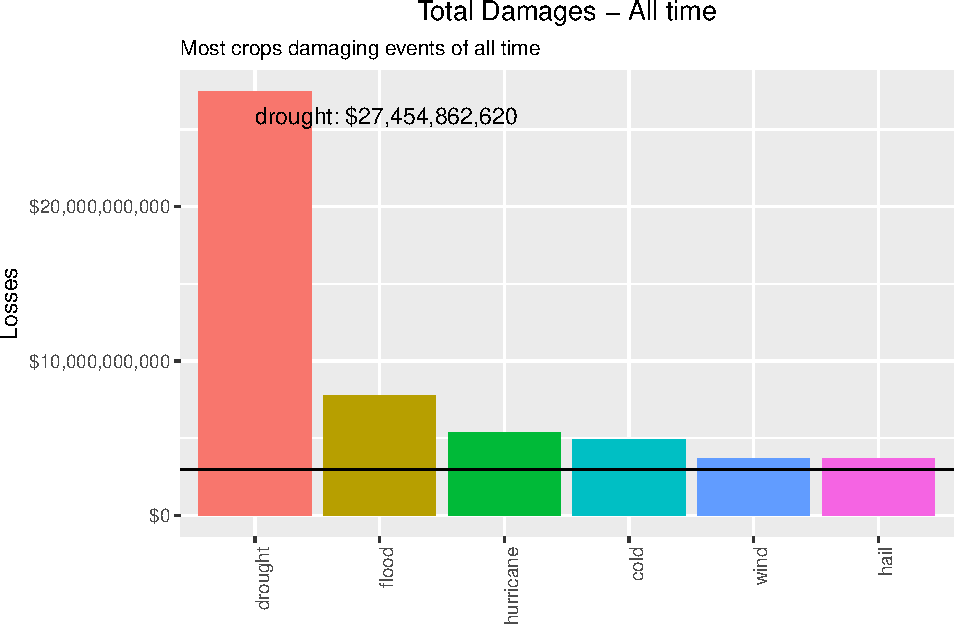
\includegraphics{readme_files/figure-latex/crop-all-plot-1.pdf}

The most crop damaging event along the time is the \textbf{DROUGHT. It
has caused \$13,972,581,000 in losses.}

Just for curiosity, lets show now what are the less damaging among the
events:

\begin{Shaded}
\begin{Highlighting}[]
\NormalTok{crop.all.df <-}\StringTok{ }\NormalTok{crop.df %>%}\StringTok{ }\KeywordTok{group_by}\NormalTok{(event) %>%}
\StringTok{                }\KeywordTok{summarise}\NormalTok{(}\DataTypeTok{total.raw =} \KeywordTok{sum}\NormalTok{(crop.ev)) %>%}
\StringTok{                }\KeywordTok{arrange}\NormalTok{(total.raw) %>%}
\StringTok{                }\KeywordTok{mutate}\NormalTok{(}\DataTypeTok{media.raw =} \KeywordTok{mean}\NormalTok{(total.raw), }
                        \DataTypeTok{mediana.raw =} \KeywordTok{median}\NormalTok{(total.raw),}
                        \DataTypeTok{total =} \KeywordTok{dollar}\NormalTok{(total.raw),}
                        \DataTypeTok{mean =} \KeywordTok{dollar}\NormalTok{(media.raw),}
                        \DataTypeTok{median =} \KeywordTok{dollar}\NormalTok{(mediana.raw),}
                        \DataTypeTok{rank =} \KeywordTok{seq}\NormalTok{(}\KeywordTok{length}\NormalTok{(event),}\DecValTok{1}\NormalTok{, }\DataTypeTok{by=}\NormalTok{-}\DecValTok{1}\NormalTok{))}



\KeywordTok{kable}\NormalTok{(crop.all.df[}\DecValTok{1}\NormalTok{:}\DecValTok{10}\NormalTok{, }\KeywordTok{c}\NormalTok{(}\DecValTok{8}\NormalTok{,}\DecValTok{1}\NormalTok{,}\DecValTok{5}\NormalTok{:}\DecValTok{7}\NormalTok{)])}
\end{Highlighting}
\end{Shaded}

\begin{longtable}[]{@{}rllll@{}}
\toprule
rank & event & total & mean & median\tabularnewline
\midrule
\endhead
22 & GUSTNADO & \$1,550 & \$2,231,988,917 & \$296,658,415\tabularnewline
21 & TSUNAMI & \$20,000 & \$2,231,988,917 & \$296,658,415\tabularnewline
20 & TYPHOON & \$825,000 & \$2,231,988,917 &
\$296,658,415\tabularnewline
19 & TIDE & \$850,000 & \$2,231,988,917 & \$296,658,415\tabularnewline
18 & LIGHTNING & \$12,092,090 & \$2,231,988,917 &
\$296,658,415\tabularnewline
17 & SLIDE & \$20,017,000 & \$2,231,988,917 &
\$296,658,415\tabularnewline
16 & WINTER & \$42,444,000 & \$2,231,988,917 &
\$296,658,415\tabularnewline
15 & FROST & \$66,000,000 & \$2,231,988,917 &
\$296,658,415\tabularnewline
14 & BLIZZARD & \$112,060,000 & \$2,231,988,917 &
\$296,658,415\tabularnewline
13 & SNOW & \$134,663,100 & \$2,231,988,917 &
\$296,658,415\tabularnewline
\bottomrule
\end{longtable}

\section{Most aflicted locations}\label{most-aflicted-locations}

Most afflicted locations

We have determined what locations had the worst outcome from those
events, both in terms of human health and economic losses.

Unfortunatelly, these has been the worst counties for living in:

\begin{Shaded}
\begin{Highlighting}[]
\CommentTok{# subset original data}
\NormalTok{cities.df <-}\StringTok{ }\NormalTok{harm.df %>%}\StringTok{ }
\StringTok{                }\KeywordTok{filter}\NormalTok{(!(}\KeywordTok{is.na}\NormalTok{(countyname) |}\StringTok{ }\KeywordTok{is.na}\NormalTok{(state))) %>%}
\StringTok{                }\KeywordTok{select}\NormalTok{(}\DecValTok{6}\NormalTok{,}\DecValTok{5}\NormalTok{,}\DecValTok{7}\NormalTok{:}\DecValTok{14}\NormalTok{) %>%}
\StringTok{                }\KeywordTok{group_by}\NormalTok{(state, countyname) %>%}
\StringTok{                }\KeywordTok{summarise}\NormalTok{(}\DataTypeTok{fatalities =} \KeywordTok{sum}\NormalTok{(fatalities, }\DataTypeTok{na.rm=}\OtherTok{TRUE}\NormalTok{),}
                        \DataTypeTok{injuries =} \KeywordTok{sum}\NormalTok{(injuries, }\DataTypeTok{na.rm=}\OtherTok{TRUE}\NormalTok{),}
                        \DataTypeTok{prop.dmg =} \KeywordTok{sum}\NormalTok{(prop.ev, }\DataTypeTok{na.rm=}\OtherTok{TRUE}\NormalTok{),}
                        \DataTypeTok{crop.dmg =} \KeywordTok{sum}\NormalTok{(crop.ev, }\DataTypeTok{na.rm=}\OtherTok{TRUE}\NormalTok{)}
                \NormalTok{)}
\end{Highlighting}
\end{Shaded}

\subsection{Worst fatality count}\label{worst-fatality-count}

\begin{Shaded}
\begin{Highlighting}[]
\NormalTok{cities.fatal.df <-}\StringTok{ }\KeywordTok{arrange}\NormalTok{(cities.df, }\KeywordTok{desc}\NormalTok{(fatalities)) %>%}\StringTok{ }\KeywordTok{ungroup}\NormalTok{(state, countyname) %>%}
\StringTok{      }\KeywordTok{mutate}\NormalTok{(}\DataTypeTok{rank =} \KeywordTok{seq_len}\NormalTok{(}\KeywordTok{length}\NormalTok{(fatalities)),}
                \DataTypeTok{prop.dmg =} \KeywordTok{dollar}\NormalTok{(prop.dmg),}
                \DataTypeTok{crop.dmg =} \KeywordTok{dollar}\NormalTok{(crop.dmg)}
             \NormalTok{)}

\KeywordTok{kable}\NormalTok{(cities.fatal.df[}\DecValTok{1}\NormalTok{:}\DecValTok{10}\NormalTok{, }\KeywordTok{c}\NormalTok{(}\DecValTok{7}\NormalTok{,}\DecValTok{1}\NormalTok{:}\DecValTok{6}\NormalTok{)])}
\end{Highlighting}
\end{Shaded}

\begin{longtable}[]{@{}rllrrll@{}}
\toprule
rank & state & countyname & fatalities & injuries & prop.dmg &
crop.dmg\tabularnewline
\midrule
\endhead
1 & IL & ILZ003 & 605 & 14 & \$429,000 & \$0\tabularnewline
2 & IL & ILZ014 & 300 & 22 & \$2,321,000 & \$0\tabularnewline
3 & PA & PAZ054 & 174 & 295 & \$124,701,980 &
\$25,000,000\tabularnewline
4 & MO & JASPER & 165 & 1271 & \$2,858,007,330 & \$5,500\tabularnewline
5 & MI & GENESEE & 121 & 925 & \$87,108,750 & \$5,000,000\tabularnewline
6 & TX & MCLENNAN & 117 & 635 & \$63,071,100 & \$4,000\tabularnewline
7 & TX & TXZ163 & 116 & 3 & \$6,131,681,000 &
\$270,200,000\tabularnewline
8 & IL & ILZ005 & 114 & 0 & \$277,000 & \$0\tabularnewline
9 & AL & JEFFERSON & 110 & 1576 & \$2,024,930,600 &
\$2,254,000\tabularnewline
10 & PA & PAZ037 & 107 & 0 & \$0 & \$0\tabularnewline
\bottomrule
\end{longtable}

\begin{Shaded}
\begin{Highlighting}[]
\NormalTok{worst.fatal.city.county <-}\StringTok{ }\NormalTok{cities.fatal.df$countyname[}\DecValTok{1}\NormalTok{]}
\NormalTok{worst.fatal.city.st <-}\StringTok{ }\NormalTok{cities.fatal.df$state[}\DecValTok{1}\NormalTok{]}
\NormalTok{worst.fatal.city.count <-}\StringTok{ }\NormalTok{cities.fatal.df$fatalities[}\DecValTok{1}\NormalTok{]}
\end{Highlighting}
\end{Shaded}

The county with the biggest fatality count is \textbf{ILZ003, in IL,
with 605 people killed.}

\subsection{Worst injuries count}\label{worst-injuries-count}

\begin{Shaded}
\begin{Highlighting}[]
\KeywordTok{rm}\NormalTok{(cities.fatal.df) }\CommentTok{# house cleanning}
\NormalTok{cities.inj.df <-}\StringTok{ }\KeywordTok{arrange}\NormalTok{(cities.df, }\KeywordTok{desc}\NormalTok{(injuries)) %>%}\StringTok{ }\KeywordTok{ungroup}\NormalTok{(state, countyname) %>%}
\StringTok{      }\KeywordTok{mutate}\NormalTok{(}\DataTypeTok{rank =} \KeywordTok{seq_len}\NormalTok{(}\KeywordTok{length}\NormalTok{(injuries)),}
                \DataTypeTok{prop.dmg =} \KeywordTok{dollar}\NormalTok{(prop.dmg),}
                \DataTypeTok{crop.dmg =} \KeywordTok{dollar}\NormalTok{(crop.dmg)}
             \NormalTok{)}

\KeywordTok{kable}\NormalTok{(cities.inj.df[}\DecValTok{1}\NormalTok{:}\DecValTok{10}\NormalTok{, }\KeywordTok{c}\NormalTok{(}\DecValTok{7}\NormalTok{,}\DecValTok{1}\NormalTok{:}\DecValTok{6}\NormalTok{)])}
\end{Highlighting}
\end{Shaded}

\begin{longtable}[]{@{}rllrrll@{}}
\toprule
rank & state & countyname & fatalities & injuries & prop.dmg &
crop.dmg\tabularnewline
\midrule
\endhead
1 & TX & WICHITA & 51 & 1852 & \$310,139,880 & \$0\tabularnewline
2 & AL & JEFFERSON & 110 & 1576 & \$2,024,930,600 &
\$2,254,000\tabularnewline
3 & OH & OHZ42 & 1 & 1568 & \$50,000,000 & \$5,000,000\tabularnewline
4 & MA & WORCESTER & 96 & 1289 & \$284,569,630 & \$0\tabularnewline
5 & OH & GREENE & 37 & 1275 & \$269,935,250 & \$0\tabularnewline
6 & MO & JASPER & 165 & 1271 & \$2,858,007,330 & \$5,500\tabularnewline
7 & MO & MOZ061 & 9 & 1133 & \$1,000 & \$0\tabularnewline
8 & AL & TUSCALOOS & 60 & 1103 & \$1,604,059,750 &
\$725,000\tabularnewline
9 & MO & MOZ009 & 73 & 978 & \$3,225,050 & \$23,649,200\tabularnewline
10 & MI & GENESEE & 121 & 925 & \$87,108,750 &
\$5,000,000\tabularnewline
\bottomrule
\end{longtable}

\begin{Shaded}
\begin{Highlighting}[]
\NormalTok{worst.inj.city.county <-}\StringTok{ }\NormalTok{cities.inj.df$countyname[}\DecValTok{1}\NormalTok{]}
\NormalTok{worst.inj.city.st <-}\StringTok{ }\NormalTok{cities.inj.df$state[}\DecValTok{1}\NormalTok{]}
\NormalTok{worst.inj.city.count <-}\StringTok{ }\NormalTok{cities.inj.df$injuries[}\DecValTok{1}\NormalTok{]}
\end{Highlighting}
\end{Shaded}

The county with the biggest injuries count is \textbf{WICHITA, in TX,
with 1852 people injuried.}

\subsection{Worst property losses}\label{worst-property-losses}

\begin{Shaded}
\begin{Highlighting}[]
\KeywordTok{rm}\NormalTok{(cities.inj.df) }\CommentTok{# house cleanning}

\NormalTok{cities.prop.df <-}\StringTok{ }\KeywordTok{arrange}\NormalTok{(cities.df, }\KeywordTok{desc}\NormalTok{(prop.dmg)) %>%}\StringTok{ }\KeywordTok{ungroup}\NormalTok{(state, countyname) %>%}
\StringTok{      }\KeywordTok{mutate}\NormalTok{(}\DataTypeTok{rank =} \KeywordTok{seq_len}\NormalTok{(}\KeywordTok{length}\NormalTok{(prop.dmg)),}
                \DataTypeTok{prop.dmg =} \KeywordTok{dollar}\NormalTok{(prop.dmg),}
                \DataTypeTok{crop.dmg =} \KeywordTok{dollar}\NormalTok{(crop.dmg)}
      \NormalTok{)}

\KeywordTok{kable}\NormalTok{(cities.prop.df[}\DecValTok{1}\NormalTok{:}\DecValTok{10}\NormalTok{, }\KeywordTok{c}\NormalTok{(}\DecValTok{7}\NormalTok{,}\DecValTok{1}\NormalTok{:}\DecValTok{6}\NormalTok{)])}
\end{Highlighting}
\end{Shaded}

\begin{longtable}[]{@{}rllrrll@{}}
\toprule
rank & state & countyname & fatalities & injuries & prop.dmg &
crop.dmg\tabularnewline
\midrule
\endhead
1 & CA & NAPA & 1 & 0 & \$115,116,385,000 & \$66,900,000\tabularnewline
2 & LA & LAZ040 & 0 & 0 & \$31,316,850,000 & \$0\tabularnewline
3 & LA & LAZ034 & 1 & 0 & \$17,152,118,400 &
\$178,330,000\tabularnewline
4 & MS & MSZ080 & 0 & 1 & \$11,264,195,000 & \$0\tabularnewline
5 & FL & FLZ068 & 19 & 16 & \$10,367,010,000 &
\$1,047,000,000\tabularnewline
6 & FL & FLZ001 & 33 & 0 & \$9,686,320,000 & \$87,800,000\tabularnewline
7 & MS & MSZ068 & 1 & 0 & \$7,375,405,000 & \$0\tabularnewline
8 & TX & TXZ163 & 116 & 3 & \$6,131,681,000 &
\$270,200,000\tabularnewline
9 & MS & MSZ018 & 17 & 104 & \$5,908,768,000 &
\$1,514,706,500\tabularnewline
10 & FL & FLZ055 & 9 & 786 & \$5,424,027,000 &
\$292,000,000\tabularnewline
\bottomrule
\end{longtable}

\begin{Shaded}
\begin{Highlighting}[]
\NormalTok{worst.prop.city.county <-}\StringTok{ }\NormalTok{cities.prop.df$countyname[}\DecValTok{1}\NormalTok{]}
\NormalTok{worst.prop.city.st <-}\StringTok{ }\NormalTok{cities.prop.df$state[}\DecValTok{1}\NormalTok{]}
\NormalTok{worst.prop.city.count <-}\StringTok{ }\NormalTok{cities.prop.df$prop.dmg[}\DecValTok{1}\NormalTok{]}
\end{Highlighting}
\end{Shaded}

The county with the biggest property losses is \textbf{NAPA, in CA, with
\$115,116,385,000 in losses.}

\subsection{Worst crops losses}\label{worst-crops-losses}

\begin{Shaded}
\begin{Highlighting}[]
\KeywordTok{rm}\NormalTok{(cities.prop.df) }\CommentTok{# house cleanning}


\NormalTok{cities.crop.df <-}\StringTok{ }\KeywordTok{arrange}\NormalTok{(cities.df, }\KeywordTok{desc}\NormalTok{(crop.dmg)) %>%}\StringTok{ }\KeywordTok{ungroup}\NormalTok{(state, countyname) %>%}
\StringTok{      }\KeywordTok{mutate}\NormalTok{(}\DataTypeTok{rank =} \KeywordTok{seq_len}\NormalTok{(}\KeywordTok{length}\NormalTok{(crop.dmg)),}
                \DataTypeTok{prop.dmg =} \KeywordTok{dollar}\NormalTok{(prop.dmg),}
                \DataTypeTok{crop.dmg =} \KeywordTok{dollar}\NormalTok{(crop.dmg)}
      \NormalTok{)}

\KeywordTok{kable}\NormalTok{(cities.crop.df[}\DecValTok{1}\NormalTok{:}\DecValTok{10}\NormalTok{, }\KeywordTok{c}\NormalTok{(}\DecValTok{7}\NormalTok{,}\DecValTok{1}\NormalTok{:}\DecValTok{6}\NormalTok{)])}
\end{Highlighting}
\end{Shaded}

\begin{longtable}[]{@{}rllrrll@{}}
\toprule
rank & state & countyname & fatalities & injuries & prop.dmg &
crop.dmg\tabularnewline
\midrule
\endhead
1 & IL & ADAMS & 0 & 23 & \$5,009,087,550 &
\$5,000,084,000\tabularnewline
2 & MS & MSZ001 & 4 & 5 & \$2,643,000 & \$5,000,000,000\tabularnewline
3 & TX & TXZ091 & 69 & 224 & \$182,509,000 &
\$2,422,471,000\tabularnewline
4 & TX & TXZ021 & 2 & 4 & \$12,450,000 & \$1,845,050,000\tabularnewline
5 & IA & IAZ004 & 10 & 9 & \$737,543,460 &
\$1,579,805,100\tabularnewline
6 & MS & MSZ018 & 17 & 104 & \$5,908,768,000 &
\$1,514,706,500\tabularnewline
7 & FL & FLZ068 & 19 & 16 & \$10,367,010,000 &
\$1,047,000,000\tabularnewline
8 & GA & GAZ001 & 20 & 29 & \$158,011,850 & \$926,260,000\tabularnewline
9 & NE & NEZ039 & 4 & 14 & \$22,057,020 & \$771,550,000\tabularnewline
10 & NC & NCZ029 & 29 & 201 & \$1,940,635,500 &
\$768,600,000\tabularnewline
\bottomrule
\end{longtable}

\begin{Shaded}
\begin{Highlighting}[]
\NormalTok{worst.crop.city.county <-}\StringTok{ }\NormalTok{cities.crop.df$countyname[}\DecValTok{1}\NormalTok{]}
\NormalTok{worst.crop.city.st <-}\StringTok{ }\NormalTok{cities.crop.df$state[}\DecValTok{1}\NormalTok{]}
\NormalTok{worst.crop.city.count <-}\StringTok{ }\NormalTok{cities.crop.df$crop.dmg[}\DecValTok{1}\NormalTok{]}
\end{Highlighting}
\end{Shaded}

The county with the biggest croperty losses is \textbf{ADAMS, in IL,
with \$5,000,084,000 in losses.}

\section{Results}\label{results}

\subsection{Population Health}\label{population-health}

\begin{Shaded}
\begin{Highlighting}[]
\CommentTok{# plist <- list(plt.fatal.single, plt.fatal.all, plt.inj.single, plt.inj.all)}
\CommentTok{# n <- length(plist)}
\CommentTok{# nCol <- floor(sqrt(n))}
\CommentTok{# do.call("grid.arrange", c(plist, ncol=nCol))}

\KeywordTok{grid.arrange}\NormalTok{(plt.fatal.single, plt.fatal.all, plt.inj.single, plt.inj.all, }
             \DataTypeTok{nrow=}\DecValTok{2}\NormalTok{, }\DataTypeTok{ncol=}\DecValTok{2}\NormalTok{,}
             \DataTypeTok{bottom=}\StringTok{"Health impact"}\NormalTok{)}
\KeywordTok{grid.rect}\NormalTok{(}\DataTypeTok{gp=}\KeywordTok{gpar}\NormalTok{(}\DataTypeTok{fill=}\OtherTok{NA}\NormalTok{))}
\end{Highlighting}
\end{Shaded}

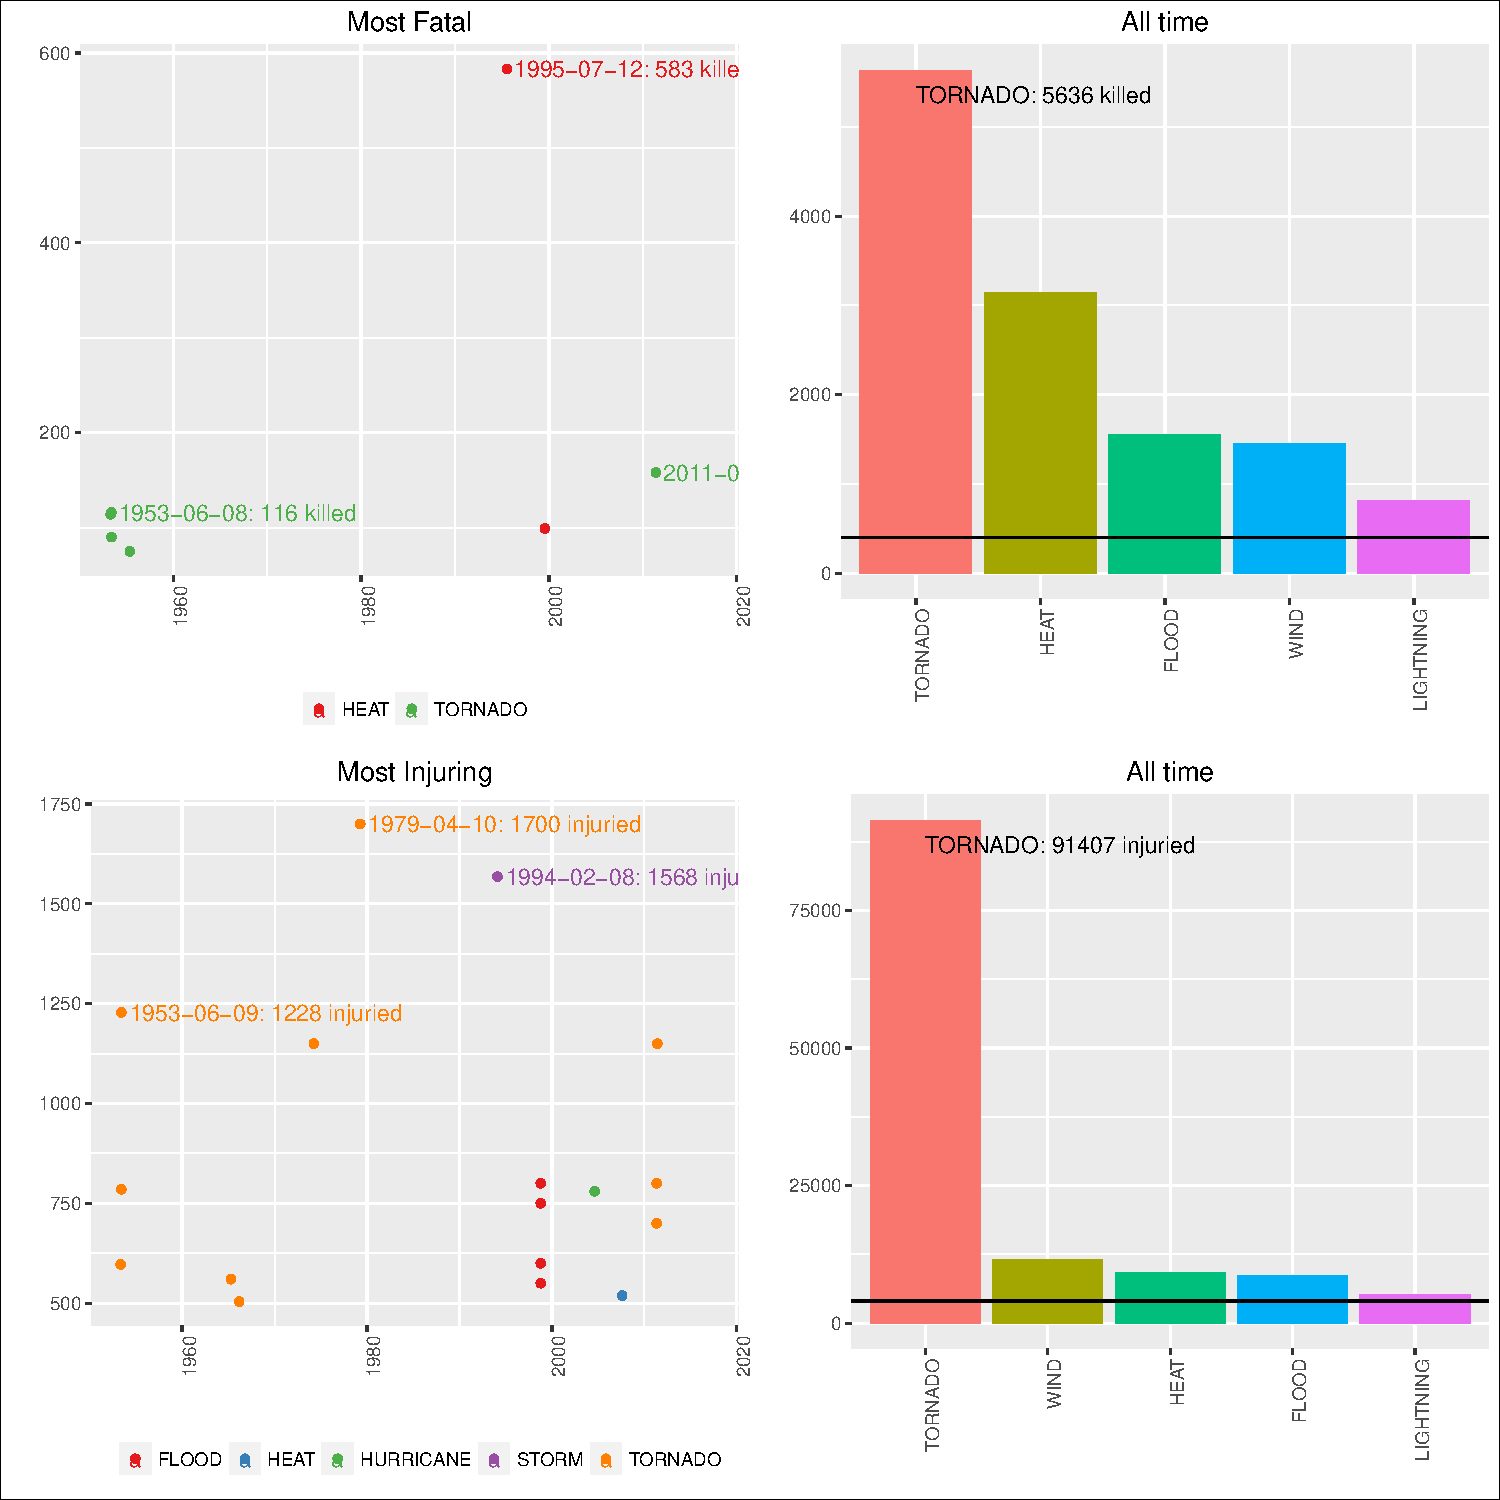
\includegraphics{readme_files/figure-latex/health-plot-1.pdf}

The single most fatal event was a \textbf{HEAT, that occurred in IL,
ILZ003, on 1995-07-12, killing 583 people.}

The most fatal event along the time is the \textbf{TORNADO. It has
killed 5636 people until now.}

The single most injuring event was a \textbf{TORNADO, that occurred in
TX, WICHITA, on 1979-04-10, injuring 1700 people.}

The most injuring event along the time is the \textbf{TORNADO. It has
injuried 91407 people until now.}

\subsection{Economic Damages}\label{economic-damages}

\begin{Shaded}
\begin{Highlighting}[]
\KeywordTok{grid.arrange}\NormalTok{(plt.prop.single, plt.prop.all,}
             \NormalTok{plt.crop.single, plt.crop.all,}
             \DataTypeTok{nrow=}\DecValTok{2}\NormalTok{, }\DataTypeTok{ncol=}\DecValTok{2}\NormalTok{,}
             \DataTypeTok{bottom=}\StringTok{"Economic impact"}\NormalTok{)}
\KeywordTok{grid.rect}\NormalTok{(}\DataTypeTok{gp=}\KeywordTok{gpar}\NormalTok{(}\DataTypeTok{fill=}\OtherTok{NA}\NormalTok{))}
\end{Highlighting}
\end{Shaded}

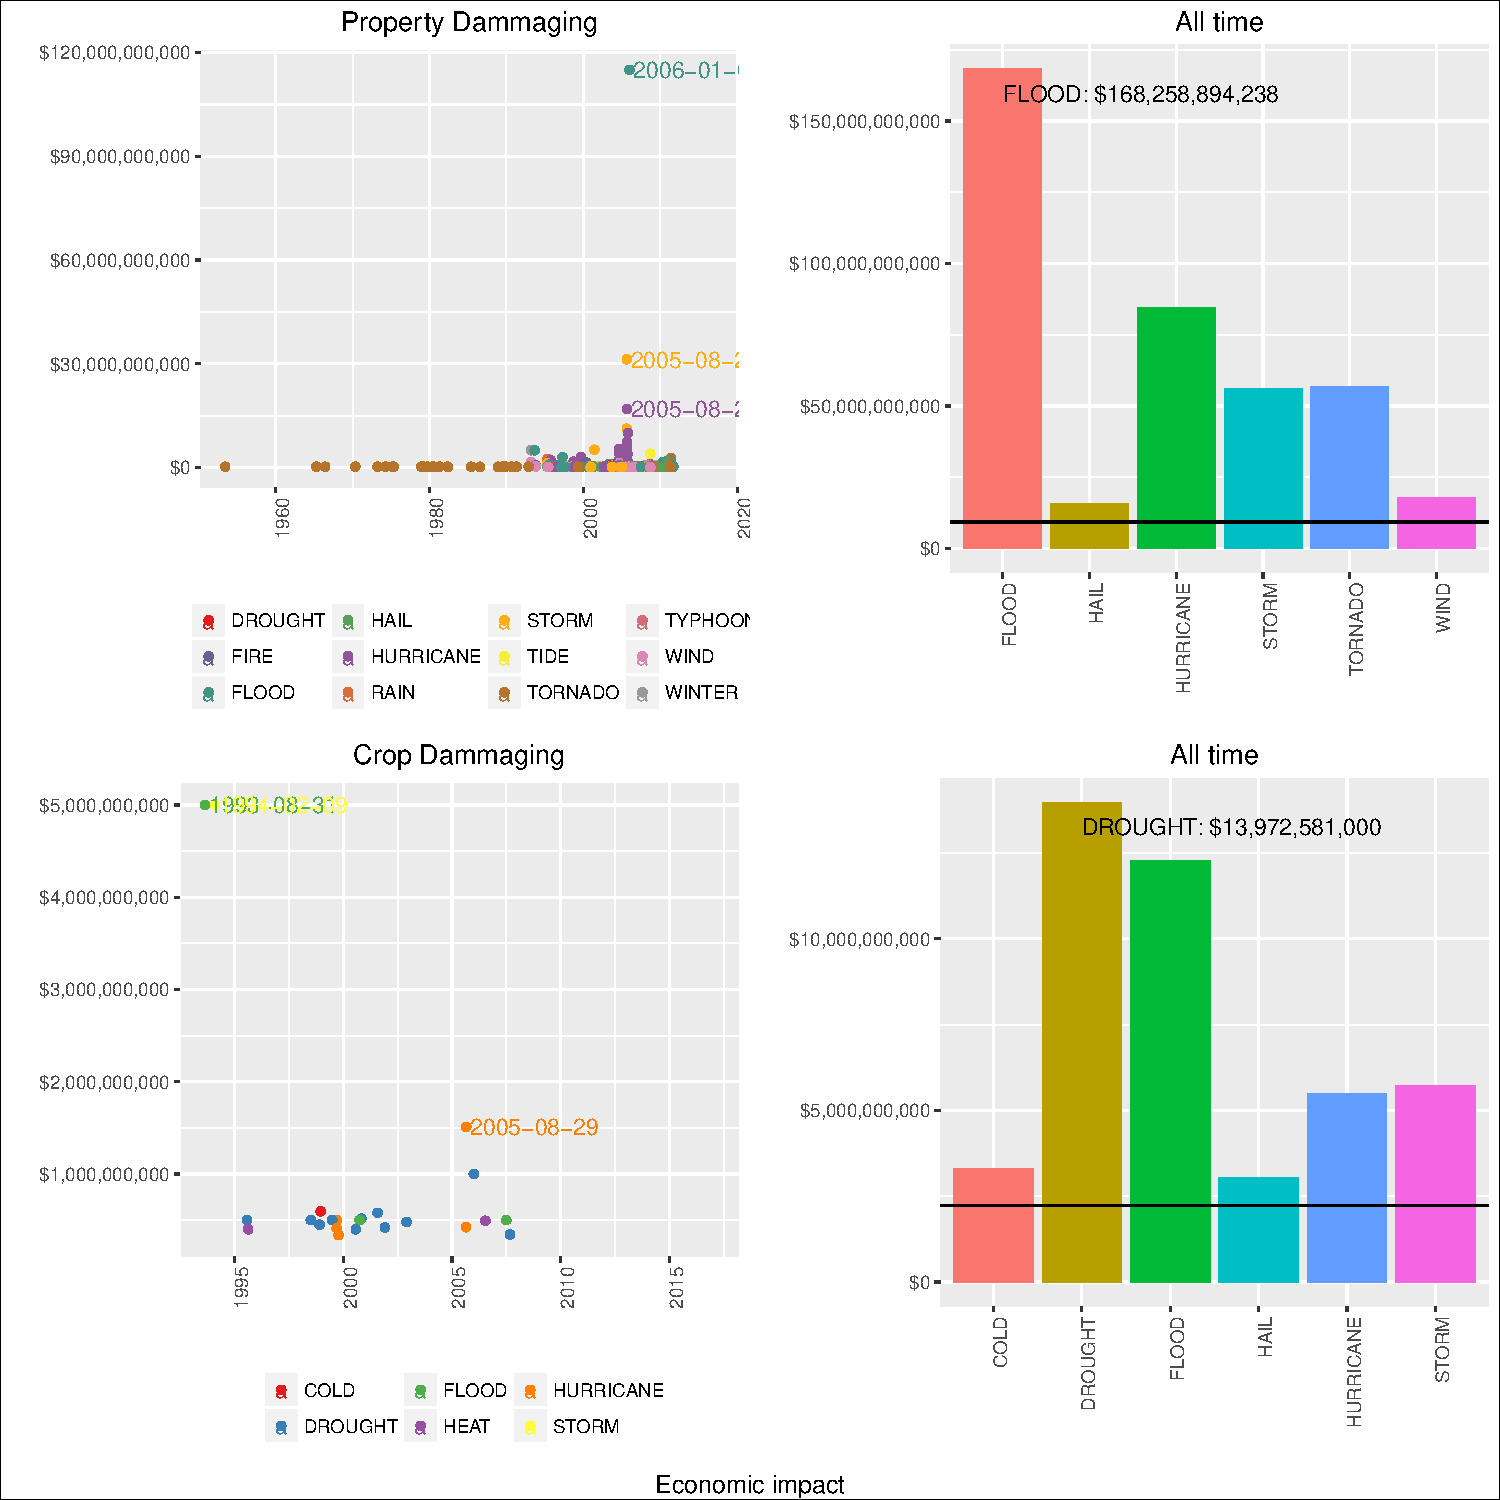
\includegraphics{readme_files/figure-latex/economic-plot-1.pdf}

The single most economic damaging event to properties was a
\textbf{FLOOD, that occurred in CA, NAPA, on 2006-01-01, causing U\$
\$115,000,000,000 in losses}.

The most property damaging event along the time is the \textbf{FLOOD. It
has caused \$168,258,894,238 in losses.}

The single most economic damaging event to crops was a \textbf{FLOOD,
that occurred in IL, ADAMS, on 1993-08-31, causing U\$ \$5,000,000,000
in losses}.

The most crop damaging event along the time is the \textbf{DROUGHT. It
has caused \$13,972,581,000 in losses.}

\subsection{Most aflicted locations}\label{most-aflicted-locations-1}

The county with the biggest fatality count is \textbf{ILZ003, in IL,
with 605 people killed.}

The county with the biggest injuries count is \textbf{WICHITA, in TX,
with 1852 people injuried.}

The county with the biggest property losses is \textbf{NAPA, in CA, with
\$115,116,385,000 in losses.}

The county with the biggest croperty losses is \textbf{ADAMS, in IL,
with \$5,000,084,000 in losses.}

\subsection{Distribution of data}\label{distribution-of-data}

\begin{Shaded}
\begin{Highlighting}[]
\KeywordTok{grid.arrange}\NormalTok{(plt.distr.fatal0, plt.distr.fatal1, plt.distr.inj0, plt.distr.inj1, }
             \DataTypeTok{nrow=}\DecValTok{1}\NormalTok{, }\DataTypeTok{ncol=}\DecValTok{4}\NormalTok{, }
             \DataTypeTok{bottom=}\StringTok{"Population distribution - fatalities and injuries"}\NormalTok{)}
\KeywordTok{grid.rect}\NormalTok{(}\DataTypeTok{gp=}\KeywordTok{gpar}\NormalTok{(}\DataTypeTok{fill=}\OtherTok{NA}\NormalTok{))             }
\end{Highlighting}
\end{Shaded}

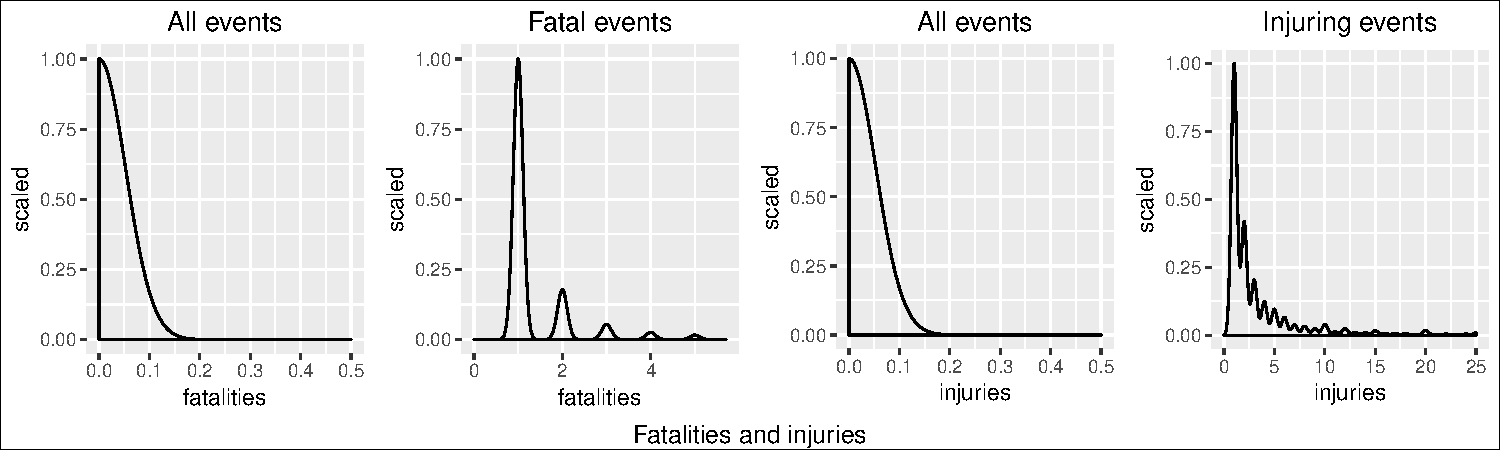
\includegraphics{readme_files/figure-latex/distribution-1.pdf}

\begin{Shaded}
\begin{Highlighting}[]
\KeywordTok{grid.arrange}\NormalTok{(plt.distr.prop0, plt.distr.prop1, plt.distr.crop0, plt.distr.crop1, }
             \DataTypeTok{nrow=}\DecValTok{1}\NormalTok{, }\DataTypeTok{ncol=}\DecValTok{4}\NormalTok{, }
             \DataTypeTok{bottom=}\StringTok{"Population distribution - property and crops losses"}\NormalTok{)}
\KeywordTok{grid.rect}\NormalTok{(}\DataTypeTok{gp=}\KeywordTok{gpar}\NormalTok{(}\DataTypeTok{fill=}\OtherTok{NA}\NormalTok{))   }
\end{Highlighting}
\end{Shaded}

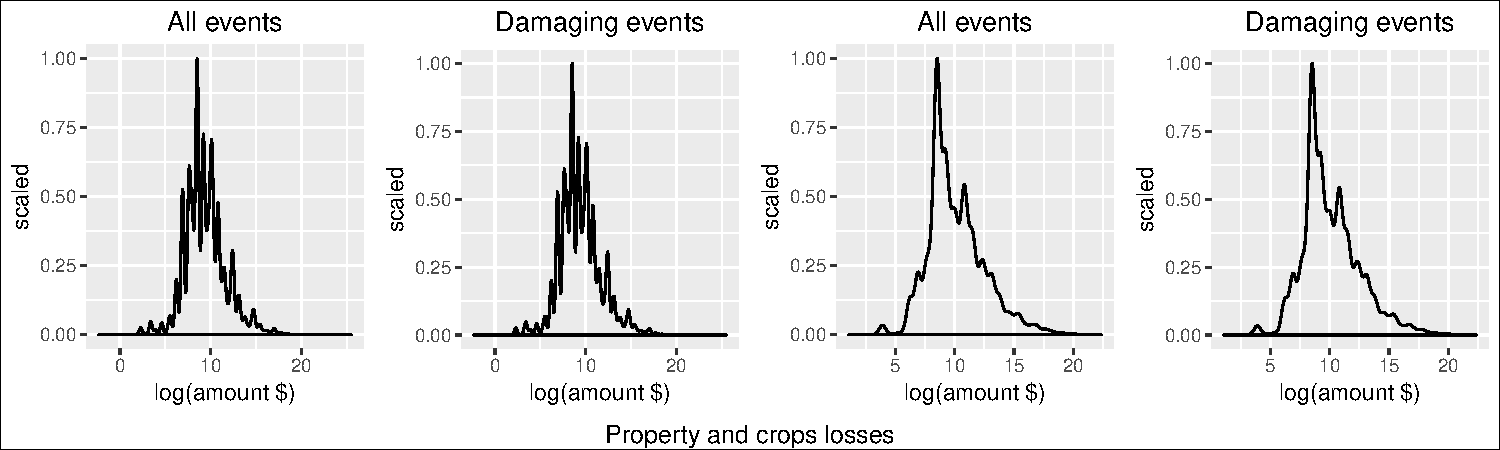
\includegraphics{readme_files/figure-latex/distribution-2.pdf}


\end{document}
